\documentclass[12pt,twoside,notitlepage]{report}
\usepackage[utf8]{inputenc}
\usepackage{tikz}
\usepackage{float}
\usepackage[ruled,vlined,noend]{algorithm2e}
\usepackage{caption}
\usepackage{subcaption}
\usepackage[english]{babel}
\usepackage{amssymb}
\usepackage{amsmath}
\DeclareMathOperator*{\argmin}{argmin}

\usepackage{tikz-uml}
\usepackage{graphicx}
\usepackage{fancybox}
\newcommand{\shadowpicture}[1]{%
  \shadowsize=1pt
  \fboxrule=0pt
  \fboxsep=0pt
  \color{gray}
  \shadowbox{\fboxsep=6pt\fcolorbox{white}{white}{#1}}
  \normalcolor
}

\usepackage{xcolor}
\usepackage{listings}
\lstset{language=java, frame=single,framesep=\fboxsep,framerule=\fboxrule,
rulecolor=\color{red},backgroundcolor=\color{yellow!5},basicstyle=\footnotesize\tt,tabsize=1,
numbersep=5mm, numbers=left,numberstyle=\footnotesize,keywordstyle=\color{blue}\sf,identifierstyle=\color{magenta}}


\begin{document}

%%%%%%%%%%%%%%%%%%%%%%%%%%%%%%%%%%%%%%%%%%%%%%%%%%%%%%%%%%%%%%%%%%%%%%%%
% Title


\pagestyle{empty}

\hfill{\LARGE \bf Oliver Freeman}

\vspace*{60mm}
\begin{center}
\Huge
{\bf A Comparison of Any-Angle Pathfinding Algorithms for Virtual Agents} \\
\vspace*{5mm}
Computer Science: Part II \\
\vspace*{5mm}
Clare College \\
\vspace*{5mm}
\today  % today's date
\end{center}

\cleardoublepage

%%%%%%%%%%%%%%%%%%%%%%%%%%%%%%%%%%%%%%%%%%%%%%%%%%%%%%%%%%%%%%%%%%%%%%%%%%%%%%
% Proforma, table of contents and list of figures

\setcounter{page}{1}
\pagenumbering{roman}
\pagestyle{plain}

\chapter*{Proforma}

{\large
\begin{tabular}{ll}
Name:               & \bf Oliver Freeman                      \\
College:            & \bf Clare College                    \\
Project Title:      & \bf A Comparison of Any-Angle Pathfinding\\ 
                    & \bf Algorithms for Virtual Agents \\
Examination:        & \bf Computer Science Tripos: Part II, May 2014        \\
Word Count:         & \bf ????\footnote{This word count was computed by ...}  \\
Project Originator: & \bf Oliver Freeman                   \\
Supervisor:         & \bf Dr R. J. Gibbens                   \\ 
\end{tabular}
}


\section*{Original Aims of the Project}

To do.


\section*{Work Completed}

To do.

\section*{Special Difficulties}

None
 
\newpage
\section*{Declaration}

I, Oliver Freeman of Clare College, being a candidate for Part II of the Computer
Science Tripos, hereby declare that this dissertation and the work described in it are my own work,
unaided except as may be specified below, and that the dissertation
does not contain material that has already been used to any substantial
extent for a comparable purpose.

\bigskip
\leftline{Signed [signature]}

\medskip
\leftline{Date [date]}

\cleardoublepage

\tableofcontents

\listoffigures

\newpage
\section*{Acknowledgements}

To do.

%%%%%%%%%%%%%%%%%%%%%%%%%%%%%%%%%%%%%%%%%%%%%%%%%%%%%%%%%%%%%%%%%%%%%%%
% now for the chapters

\cleardoublepage        % just to make sure before the page numbering
                        % is changed

\setcounter{page}{1}
\pagenumbering{arabic}
\pagestyle{headings}

\chapter{Introduction}

\section{Motivation}

Finding short and realistic-looking paths through environments with arbitrarily placed obstacles is one of the central problems in artificial intelligence for games and robotics.\\

\noindent
Pathfinding algorithms operate on a discrete mathematical construct called a graph. Therefore, to find a path through a continuous environment, the robot must obtain a graph that is a simplified representation of the environment - it is a simplification because it represents a continuous space environment with a discrete, finite object. Studies comparing algorithms for finding paths through graphs have shown that A* finds the optimal path in consistently less time than other pathfinding algorithms [Dagys 2013]. However, although the paths are optimal with respect to the graph, they are rarely optimal with respect to the environment (see Figure 1.1).\\

\noindent
Over the last few years there have been multiple new algorithms proposed to efficiently find optimal or near-optimal paths through continuous environments. This dissertation aims to investigate their relative merits.

\begin{figure}
  \begin{subfigure}{.4\textwidth}
    \centering
    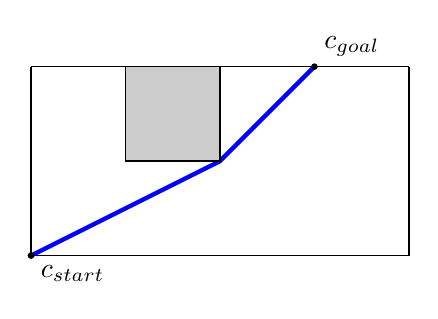
\begin{tikzpicture}[scale=1.2,line width=0.5pt]
    
      \draw[black] (0,0) -- (4,0);
      \draw[black] (0,0) -- (0,2);
      \draw[black] (4,2) -- (4,0);
      \draw[black] (4,2) -- (0,2);

      \node[above right] at (3,2) {$c_{goal}$};
      \node[below right] at (0,0) {$c_{start}$};

      \draw[blue, ultra thick] (0,0) -- (2,1) -- (3,2);
      \filldraw[color=black,fill=black!20] (1,1) rectangle (2,2);  
      \fill (0,0) circle (1pt);
      \fill (3,2) circle (1pt);

    \end{tikzpicture}
    \caption{Environment}
    %\label{fig:sfi2}
  \end{subfigure}
  %
  \begin{subfigure}{.4\textwidth}
    \centering
    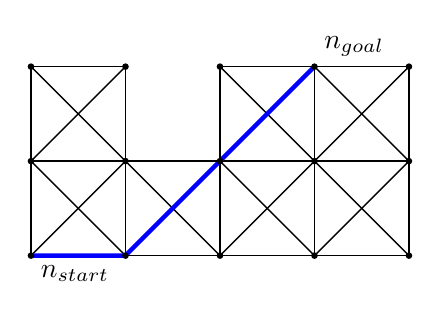
\begin{tikzpicture}[scale=1.2,line width=0.5pt]
      \draw[black] (0,0) grid (4,2);
  
      \foreach \x in {0,1,2,3} {
        \foreach \y in {0,1} {
          \pgfmathparse{int(\x + 1)};
          \let\xa\pgfmathresult;
          \pgfmathparse{int(\y + 1)};
          \let\ya\pgfmathresult;
          \draw[black] (\x,\y) -- (\xa,\ya);
        }
      }
  
      \foreach \x in {0,1,2,3} {
        \foreach \y in {1,2} {
          \pgfmathparse{int(\x + 1)};
          \let\xa\pgfmathresult;
          \pgfmathparse{int(\y - 1)};
          \let\ya\pgfmathresult;
          \draw[black] (\x,\y) -- (\xa,\ya);
        }
      }

      \node[above right] at (3,2) {$n_{goal}$};
      \node[below right] at (0,0) {$n_{start}$};

      \draw[blue, ultra thick] (0,0) -- (1,0) -- (3,2);
      
      \filldraw[color=black,fill=white] (1,1) rectangle (2,2);
      \draw[white, ultra thick] (1,2) -- (2,2);

      \foreach \x in {0,1,2,3,4} {
        \foreach \y in {0,1,2} {
          \fill (\x,\y) circle (1pt);
        }e
      }
    \end{tikzpicture}
    \caption{Graph}
    %\label{fig:sfig1}
  \end{subfigure}
  \caption{Shortest path through environment vs. shortest path through graph}
  %\label{fig:fig}
\end{figure}

\section{Related work}

To do.

\section {Project goals}

To do.

\cleardoublepage


\chapter{Preparation} 

\section{Introduction to any-angle pathfinding}

In this section I will introduce some key terms, define the any-angle pathfinding problem, and describe some decisions and methods to solve the problem.

\subsection{Definitions}

\begin{description}
\item[Agent] \hfill \\
  An entity that can move from one location in the environment to another. The agent cannot move to or through a location that is blocked by an obstacle.
  \item[Map] \hfill \\
  A representation of an environment as a two dimensional plane {$\mathbb{R}^{2}$}. For simplicity, this dissertation will focus on grid-based maps, where a map is divided into {$N^{2}$} cells of equal size. 
    \item[Cell] \hfill \\
  The logical unit of a map. Each cell may either be free or blocked. A blocked cell represents an obstacle that completely fills the cell.
  \item[Line of Sight] \hfill \\
  Exists between two coordinates on a map if a straight line between those two coordinates does not intersect any blocked cells.
   \item[Path] \hfill \\
  An ordered list of coordinates ({$c_{start}$}, {$c_{1}$}, ..., {$c_{goal}$}). For the path to be valid, a line of sight must exist between {$c_{start}$} and {$c_{1}$}, {$c_{1}$} and {$c_{2}$}, ... {$c_{n-1}$} and {$c_{goal}$}.
  \item[Graph] \hfill \\
  A finite mathematical construct, consisting of nodes and undirected edges. A graph is a discrete representation of the {$\mathbb{R}^{2}$} space of the map.
  \item[Node] \hfill \\
  Represents a single $coordinate$ on the map.
  \item[Edge] \hfill \\
  An unordered pair of nodes. The existence of edge ({$n_{1}$},{$n_{2}$}) denotes that an agent can travel in a straight line between the coordinates represented by {$n_{1}$} and {$n_{2}$}. Each edge has an associated $weight$, which represents the Euclidean distance between the coordinates represented by the two nodes.
    \item[Neighbour] \hfill \\
    A node {$n'$} is the neighbour of a node {$n$} if there exists an edge ({$n$},{$n'$}).
  
\end{description}

\subsection{The any-angle pathfinding problem}

The problem is to compute optimal or near-optimal paths, if they exist, through maps. The optimality is based on the total Euclidean distance and cumulative angle turned by an agent following the path. \\

\noindent
The problem is split into two sub-problems:
\begin{itemize}
\item {\em Discretization} - a graph is created that represents that map in some way
\item {\em Pathfinding} - an algorithm is run on the graph to produce a path
\end{itemize}

These two sub-problems will now be introduced:

\subsection{Discretization}

We must choose how to represent a continuous space, grid-based map with a graph consisting of a finite number of nodes and edges.\\

\noindent
{\bfseries Grid-based graph}\\

\noindent
A common representation is to use a grid-based graph: there is one node per cell, and there are edges between nodes that represent locations that can be reached in a {$1$} unit step at {$0^{o}$}, {$90^{o}$}, {$180^{o}$} or {$270^{o}$} bearing, or a {$\sqrt{2}$} step at {$45^{o}$}, {$135^{o}$}, {$225^{o}$} or {$315^{o}$} bearing. If the location represented by one node cannot be reached from the location represented by another node (because there is a blocked cell in between), then there will be no edge between the two nodes. We are now presented with a choice as to where to place the nodes:

\begin{figure}[h]
  \begin{subfigure}{.5\textwidth}
    \centering
    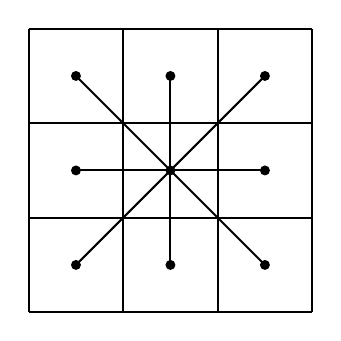
\begin{tikzpicture}[scale=1.2,line width=0.75pt]
      \draw[black] (0,0) grid (3,3);
      
      \fill[black] (0.5,0.5) circle (1.5pt);
      \fill[black] (0.5,1.5) circle (1.5pt);
      \fill[black] (0.5,2.5) circle (1.5pt);
      \fill[black] (1.5,0.5) circle (1.5pt);
      \fill[black] (1.5,1.5) circle (1.5pt);
      \fill[black] (1.5,2.5) circle (1.5pt);
      \fill[black] (2.5,0.5) circle (1.5pt);
      \fill[black] (2.5,1.5) circle (1.5pt);
      \fill[black] (2.5,2.5) circle (1.5pt);
      
      \draw[black] (1.5,1.5) -- (0.5,0.5);
      \draw[black] (1.5,1.5) -- (0.5,1.5);
      \draw[black] (1.5,1.5) -- (0.5,2.5);
      \draw[black] (1.5,1.5) -- (1.5,0.5);
      \draw[black] (1.5,1.5) -- (1.5,2.5);
      \draw[black] (1.5,1.5) -- (2.5,0.5);
      \draw[black] (1.5,1.5) -- (2.5,1.5);
      \draw[black] (1.5,1.5) -- (2.5,2.5);
     
    \end{tikzpicture}
    \caption{Nodes in the centres of cells}
    %\label{fig:sfig1}
  \end{subfigure}
  %
  \begin{subfigure}{.5\textwidth}
    \centering
    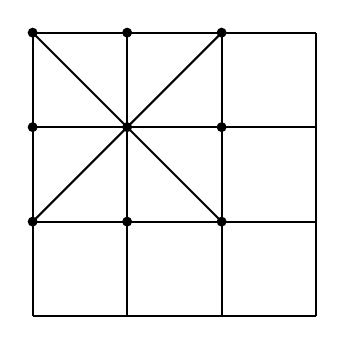
\begin{tikzpicture}[scale=1.2,line width=0.75pt]
      
      \draw[black] (0,0) grid (3,3);
      
      \fill[black] (0,3) circle (1.5pt);
      \fill[black] (1,3) circle (1.5pt);
      \fill[black] (2,3) circle (1.5pt);
      \fill[black] (0,2) circle (1.5pt);
      \fill[black] (1,2) circle (1.5pt);
      \fill[black] (2,2) circle (1.5pt);
      \fill[black] (0,1) circle (1.5pt);
      \fill[black] (1,1) circle (1.5pt);
      \fill[black] (2,1) circle (1.5pt);
      
      \draw[black] (1,2) -- (0,3);
      \draw[black] (1,2) -- (1,3);
      \draw[black] (1,2) -- (2,3);
      \draw[black] (1,2) -- (0,2);
      \draw[black] (1,2) -- (2,2);
      \draw[black] (1,2) -- (0,1);
      \draw[black] (1,2) -- (1,1);
      \draw[black] (1,2) -- (2,1);
      
    \end{tikzpicture}
    \caption{Nodes on the corners of cells}
    %\label{fig:sfi2}
  \end{subfigure}
  \caption{A node and its eight neighbours}
  %\label{fig:fig}
\end{figure}

\noindent
The choice is essentially a stylistic one for most of the algorithms, but placing nodes in the middle of cells places stringent restrictions on the paths produced by Block A*, so I will place my nodes on the corners of cells. \\

\noindent
{\bfseries Visibility graph}\\

\noindent
This is an alternative graph representation. Nodes exist at the start and end coordinates, and otherwise only on the corner of cells for which exactly three of the four surrounding cells are free. An edge exists between any two nodes that have a line of sight.\\

\begin{figure}[h]
\begin{subfigure}{.3\textwidth}
    \centering
    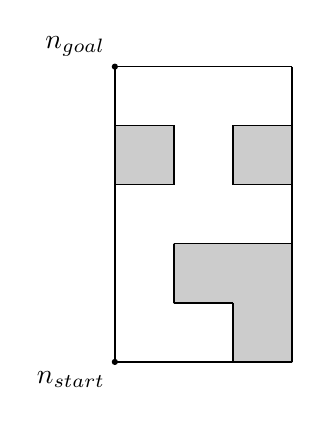
\begin{tikzpicture}[scale=0.75,line width=0.5pt]

      \node[below left] at (0,0) {$n_{start}$};
      \fill (0,0) circle (1.5pt);
      \node[above left] at (0,5) {$n_{goal}$};
      \fill (0,5) circle (1.5pt);
      
      \filldraw[color=black,fill=black!20] (0,3) rectangle (1,4);
      \filldraw[color=black,fill=black!20] (2,3) rectangle (3,4);
      \filldraw[color=black!20,fill=black!20] (1,1) rectangle (2,2);
      \filldraw[color=black!20,fill=black!20] (2,0) rectangle (3,2);
      \draw (1,1) -- (1,2);
      \draw (1,1) -- (2,1);
      \draw (1,2) -- (3,2);
      \draw (2,1) -- (2,0);
      \draw[black] (0,0) -- (3,0);
      \draw[black] (0,0) -- (0,5);
      \draw[black] (3,5) -- (3,0);
      \draw[black] (3,5) -- (0,5);
      
    \end{tikzpicture}
    \caption{Map}
    %\label{fig:sfig1}
  \end{subfigure}
  \begin{subfigure}{.3\textwidth}
    \centering
    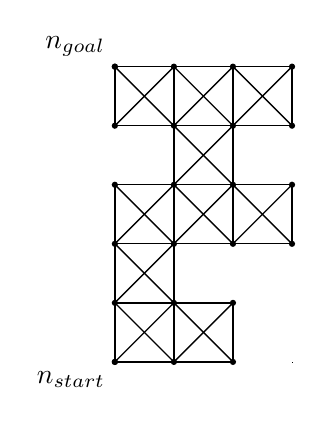
\begin{tikzpicture}[scale=0.75,line width=0.5pt]
      \draw[black] (0,0) grid (3,5);
      
      \node[below left] at (0,0) {$n_{start}$};
      \fill (0,0) circle (1.5pt);
      \node[above left] at (0,5) {$n_{goal}$};
      \fill (0,5) circle (1.5pt);
      
      
       \foreach \x in {0,1,2} {
        \foreach \y in {0,1,2,3,4} {
          \pgfmathparse{int(\x + 1)};
          \let\xa\pgfmathresult;
          \pgfmathparse{int(\y + 1)};
          \let\ya\pgfmathresult;
          \draw[black] (\x,\y) -- (\xa,\ya);
        }
      }
  
      \foreach \x in {0,1,2} {
        \foreach \y in {1,2,3,4,5} {
          \pgfmathparse{int(\x + 1)};
          \let\xa\pgfmathresult;
          \pgfmathparse{int(\y - 1)};
          \let\ya\pgfmathresult;
          \draw[black] (\x,\y) -- (\xa,\ya);
        }
      }
      
      \filldraw[color=black,fill=white] (1,1) rectangle (2,2);
      \filldraw[color=black,fill=white] (2,0) rectangle (3,2);
      \filldraw[color=black,fill=white] (0,3) rectangle (1,4);
      \filldraw[color=black,fill=white] (2,3) rectangle (3,4);
      \draw[white,ultra thick] (2,0) -- (3,0);
      \draw[white,ultra thick] (3,0) -- (3,2);
      \draw[white,ultra thick] (3,3) -- (3,4);
      \draw[white,ultra thick] (2,1) -- (2,2);
      \draw[white,ultra thick] (0,3) -- (0,4);
      
      \foreach \x in {0,1,2} {
        \foreach \y in {0,1,2,3,4,5} {
          \fill (\x,\y) circle (1.5pt);
        }
      }
      \foreach \y in {2,3,4,5} {
        \fill (3,\y) circle (1.5pt);
      }
      
    \end{tikzpicture}
    \caption{Grid-based graph}
    %\label{fig:sfig1}
  \end{subfigure}
  %
  \begin{subfigure}{.3\textwidth}
    \centering
    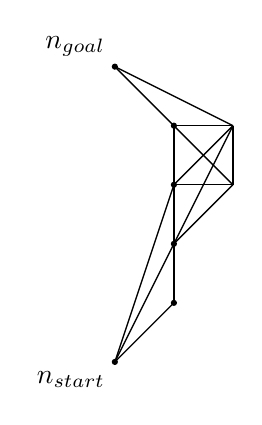
\begin{tikzpicture}[scale=0.75,line width=0.5pt]
    
      \node[below left] at (0,0) {$n_{start}$};
      \fill (0,0) circle (1.5pt);
      \node[above left] at (0,5) {$n_{goal}$};
      \fill (0,5) circle (1.5pt);
      
      \fill (1,1) circle (1.5pt);
      \fill (1,2) circle (1.5pt);
      \fill (1,3) circle (1.5pt);
      \fill (1,4) circle (1.5pt);
      \draw[black] (0,0) -- (1,1);
      \draw[black] (0,0) -- (2,4);
      \draw[black] (0,0) -- (1,3);
      \draw[black] (1,1) -- (1,4);
      \draw[black] (1,2) -- (2,3);
      \draw[black] (1,3) -- (2,3);
      \draw[black] (1,3) -- (2,4);
      \draw[black] (1,4) -- (2,3);
      \draw[black] (1,4) -- (2,4);
      \draw[black] (1,4) -- (0,5);
      \draw[black] (2,4) -- (0,5);
      \draw[black] (2,4) -- (2,3);
          
    \end{tikzpicture}
    \caption{Visibility graph}
    %\label{fig:sfi2}
  \end{subfigure}
  \caption{Different graph representations for a given map}
  %\label{fig:fig}
\end{figure}

\noindent
The optimal path through a visibility graph will correspond to the optimal path through a map, whereas the optimal path through a grid-based graph may not. However, grid-based graphs are generally accepted as preferable since, for a map of {$N^{2}$} cells, a grid-based graph will have {$O(N^{2})$} edges, whereas a visibility graph has {$O(N^{4})$} edges, which can be unfeasible for large or high resolution maps. Therefore, this investigation will focus predominantly on grid-based graphs.\\

\begin{figure}
    \centering
    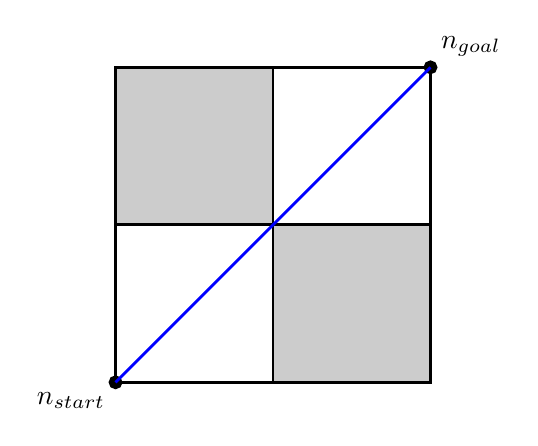
\begin{tikzpicture}[scale=2,line width=1pt]
    
      \draw (0,0) grid (2,2);
      \filldraw[color=black,fill=black!20] (0,1) rectangle (1,2); 
      \filldraw[color=black,fill=black!20] (1,0) rectangle (2,1); 
      \filldraw (0,0) circle (1pt);
      \filldraw (2,2) circle (1pt);
      \node[below left] at (0,0) {$n_{start}$};
      \node[above right] at (2,2) {$n_{goal}$};
      \draw[blue] (0,0) -- (2,2);
      
          
    \end{tikzpicture}
  \caption{A valid path for an agent modelled as a point}
  %\label{fig:fig}
\end{figure}


\noindent
{\bfseries Agent size}\\

\noindent
I will adopt the standard practice in any-angle pathfinding research by modelling the agent as a dimensionless point. Therefore, the path shown in Figure 2.3, which features a 'diagonal blockage', is a valid path. It is possible to ensure that such paths are never taken by adding extra checks in the graph creation and line of sight algorithms, but this would distract from the core investigation and be an unnecessary deviation from the accepted standard.

\section{Any-angle pathfinding algorithms}

In this section, I will introduce the four any-angle pathfinding algorithms that I will be investigating: A* with post smoothing, Theta*, Lazy Theta* and Block A*. Firstly, I will introduce an additional two comparatively basic algorithms to aid in the explanation of the more complex algorithms.

\subsection {Dijkstra's shortest paths}

Most of the algorithms that I will study will be derivatives of the well known A* graph traversal algorithm, which itself is a derivative of Dijkstra's famous shortest-path algorithm.\\

\noindent
Dijkstra finds the shortest path from a given node {$n_{start}$} to all other nodes in a graph - though it can be prematurely terminated when the goal is reached. Each node {$n$} has a:
\begin{itemize}
\item {\em g-value} - represents the length of the shortest path found so far from {$n_{start}$} to {$n$}. Initialised to $\infty$.
\item {\em parent} - the previous node in the shortest path found so far from {$n_{start}$} to {$n$}
\end{itemize}
The algorithm processes each node once only, selecting it from $openSet$, a priority queue that prioritises low g-values. When a node is selected, it's g-value is the length of the shortest path to it from {$n_{start}$}. A closed set is used to ensure that no node is expanded twice, as this would incur unnecessary work. When {$n_{goal}$} is processed, the algorithm terminates. Dijkstra's shortest-path algorithm is optimal and complete.\\

\begin{algorithm}[htp]
  \SetAlgoLined\DontPrintSemicolon
  \SetKwFunction{dijkstra}{Dijkstra}\SetKwFunction{update}{Update}
  \SetKwProg{myDef}{def}{}{}
  \myDef{\dijkstra{G, $n_{start}$, $n_{goal}$}}{
  \nl $openSet \gets \emptyset$\;
  \nl $closedSet \gets \emptyset$\;
  \nl $n_{start}.g \gets 0$\;
  \nl $openSet.add(n_{start})$\;
  \nl \While{$openSet \neq \emptyset$} {
    \nl $n_{curr} \gets openSet.pop()$\;
    \nl $closedSet.add(n_{curr})$\;
    \nl \If{$n_{curr} = n_{goal}$} {
      \nl \KwRet{$n_{goal}$}\;
    }
    \nl \ForEach{$n_{neigh}$ of $n_{curr} $} {
      \nl \If{$closedSet.contains(n_{neigh}) = false $} {
        \nl \If{$\update(n_{neigh}) = true$} {
          \nl \If{$openSet.contains(n_{neigh}) = false $} {
            \nl $openSet.add(n_{neigh})$\;
          }
        }
      }
    }
  }
  \nl \KwRet{$\emptyset$}\;
}{}
  \setcounter{AlgoLine}{0}
  \myDef{\update{$n_{neigh}$}}{
    \nl \uIf{$n_{curr}.g + euclidean(n_{curr},n_{neigh}) < n_{neigh}.g$} {
      \nl $n_{neigh}.g = n_{curr}.g + euclidean(n_{curr},n_{neigh})$\;
      \nl $n_{neigh}.parent = n_{curr}$\;
      \nl \KwRet{$true$}\;
    } \nl \Else {
      \nl \KwRet{$false$}\;
    } 
  }
  \caption{{\sc DIJKSTRA}}
\end{algorithm} 

\noindent
If a path exists, the algorithm returns $n_{goal}$. The shortest path from {$n_{start}$} to {$n_{goal}$} can be then be traced: \\({$n_{goal}$}, {$n_{goal}.parent$}, {$n_{goal}.parent.parent$}, ..., {$n_{start})$}

\subsection {A*}

A* is based on Dijkstra's shortest-path algorithm, but uses a heuristic {$h$} to reduce the number of nodes expanded, and hence often finds the optimal route to {$n_{goal}$} in less time. Where Dijkstra preferentially expands nodes with low g-values, A* preferentially expands nodes with low f-values, where {$f(n) = g(n) + h(n)$}: 
\begin{itemize}
\item {\em {$g(n)$}} - calculated in the same way as in Dijkstra's algorithm
\item {\em {$h(n)$}} - Euclidean distance between {$n$} and {$n_{goal}$}  - a cheaply computable monotonic estimate of the actual distance that will need to be traversed.
\end{itemize}
The monotonicity of Euclidean distance as a heuristic ensures that A* is optimal and complete. \\

\noindent
The pseudocode for A* differs only from Dijkstra in the {\tt update} subroutine, where the h-score must also be initialised.

\begin{algorithm}[htp]
  \SetAlgoLined\DontPrintSemicolon
  \SetKwFunction{update}{Update}
  \SetKwProg{myDef}{def}{}{}
  \myDef{\update{$n_{neigh}$}}{
    \nl \uIf{$n_{curr}.g + euclidean(n_{curr},n_{neigh}) < n_{neigh}.g$} {
      \nl $n_{neigh}.g \gets n_{curr}.g + euclidean(n_{curr},n_{neigh})$\;
      \nl $n_{neigh}.f \gets euclidean(n_{neigh},n_{goal})$\;
      \nl $n_{neigh}.parent = n_{curr}$\;
      \nl \KwRet{$true$}\;
    } \nl \Else {
      \nl \KwRet{$false$}\;
    } 
  }
  \caption{{\tt Update} from {\sc A*}}
\end{algorithm} 

\subsection {A* with post-smoothing}

A post processing step is run on the path returned by A*, where any unnecessary deviations are cut out by changing the parents of nodes of the path:

\noindent
The algorithm starts with the node returned by A*: {$ n = n_{goal}$}. The algorithm performs a line of sight test from {$n$} to {$n$}'s parent's parent. If the test passes, {$n$} will have its parent set to be its parent's parent. This test and parent resetting is repeated until the line of sight test fails. Once the test has failed, we choose a new {$n$}, which will be the old {$n$}'s parent's parent - i.e. the node on which the line of sight test failed. We repeat this process until we reach the start node, at which point the algorithm terminates.\\

\begin{figure}[h]
  \begin{subfigure}{.3\textwidth}
    \centering
    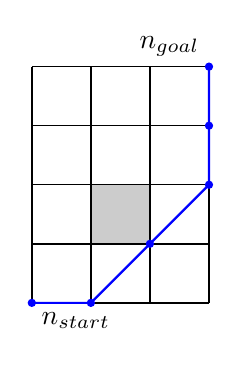
\begin{tikzpicture}[scale=0.75,line width=0.5pt, >=latex]
    
      \draw (0,0) grid (3,4);
    
      \node[below right] at (0,0) {$n_{start}$};
      \node[above left] at (3,4) {$n_{goal}$};

      \filldraw[color=black,fill=black!20] (1,1) rectangle (2,2); 
    
      \draw[blue, thick] (0,0) -- (1,0) -- (3,2) -- (3,4);
      \fill[blue,thick] (0,0) circle (2pt);
      \fill[blue,thick] (1,0) circle (2pt);
      \fill[blue,thick] (2,1) circle (2pt);
      \fill[blue,thick] (3,2) circle (2pt);
      \fill[blue,thick] (3,3) circle (2pt);
      \fill[blue,thick] (3,4) circle (2pt);

    \end{tikzpicture}
    \caption{Original path}
    %\label{fig:sfi2}
  \end{subfigure}
  \begin{subfigure}{.3\textwidth}
    \centering
    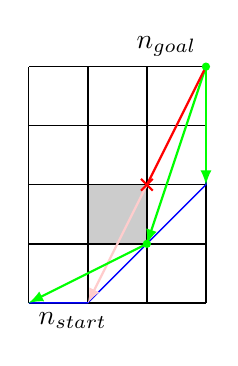
\begin{tikzpicture}[scale=0.75,line width=0.5pt, >=latex]
    
      \draw (0,0) grid (3,4);
    
      \node[below right] at (0,0) {$n_{start}$};
      \node[above left] at (3,4) {$n_{goal}$};

      \filldraw[color=black,fill=black!20] (1,1) rectangle (2,2); 
    
      \draw[blue] (0,0) -- (1,0) -- (3,2) -- (3,4);
      \draw[green, thick,->] (3,4) -- (3,2);
      \draw[green,thick,->] (3,4) -- (2,1);
      \draw[red,thick] (3,4) -- (2,2);
      \draw[red!20,thick,->] (2,2) -- (1,0);
      \draw[red,thick] (1.9,2.1) -- (2.1,1.9);
      \draw[red,thick] (1.9,1.9) -- (2.1,2.1);
      \draw[green,thick, ->] (2,1) -- (0,0);
    
      \fill[green] (3,4) circle (2pt);
      \fill[green] (2,1) circle (2pt);

    \end{tikzpicture}
    \caption{Line of sight tests} \label{fig:astarsmoothed}
  \end{subfigure}
  %
  \begin{subfigure}{.3\textwidth}
    \centering
    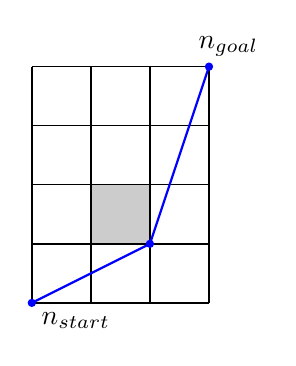
\begin{tikzpicture}[scale=0.75,line width=0.5pt, >=latex]
    
      \draw (0,0) grid (3,4);
    
      \node[below right] at (0,0) {$n_{start}$};
      \node[above left] at (4,4) {$n_{goal}$};

      \filldraw[color=black,fill=black!20] (1,1) rectangle (2,2); 
    
      \draw[blue, thick] (0,0) -- (2,1) -- (3,4);
      \fill[blue,thick] (0,0) circle (2pt);
      \fill[blue,thick] (2,1) circle (2pt);
      \fill[blue,thick] (3,4) circle (2pt);

    \end{tikzpicture}
    \caption{Improved path}
    %\label{fig:sfi2}
  \end{subfigure}
  \caption{A* with post-smoothing}
  %\label{fig:fig}
\end{figure}


\begin{algorithm}[htp]
  \SetAlgoLined\DontPrintSemicolon
  \SetKwFunction{ps}{PostSmoothing}\SetKwFunction{los}{LineOfSight}
  \SetKwProg{myDef}{def}{}{}
  \myDef{\ps{$n_{start}, n_{goal}$}}{
    \nl $n_{curr} \gets n_{goal} $\;
    \nl $n_{next} \gets n_{goal}.parent.parent $\;
    \nl \uIf {$n_{next}  = \emptyset$} {
      \nl \KwRet{} \;
    }
    \nl \While{$true$} {
      \nl \While{$\los(n_{curr} ,n_{next} )$} {
        \nl $n_{curr}.parent \gets n_{next} $\;
        \nl $n_{next}  \gets n_{next} .parent$\;
        \nl \uIf{$n_{next}  = n_{start}$} {
          \nl \KwRet{} \;
        }
      }
      \nl $n_{curr}  \gets n_{next} $\;
      \nl \uIf{$n_{curr}.parent = n_{start}$} {
        \nl \KwRet{}\;
        }
      \nl $n_{next}  \gets n_{next}.parent.parent$\;
    }
  }
  \caption{{\tt PostSmoothing} from {\sc A* with post-smoothing}}
\end{algorithm} 

\subsection {Basic {$\theta^{*}$}}

Where A* with post-smoothing does an explicit smoothing step after finding the basic path, Basic {$\theta^{*}$} interleaves smoothing with exploration by attempting to re-parent each node that is expanded with the parent of its parent. This reparenting occurs if there exists a line of sight between the node being expanded and the parent of its parent.\\

\begin{algorithm}[htp]
  \SetAlgoLined\DontPrintSemicolon
  \SetKwFunction{update}{Update}\SetKwFunction{los}{LineOfSight}
  \SetKwProg{myDef}{def}{}{}
  \myDef{\update{$n_{neigh}$}}{
    \nl \uIf{$\los(n_{neigh}, n_{curr}.parent) = true$} {
      \nl \uIf{$n_{curr}.parent.g + euclidean(n_{curr}.parent,n_{neigh}) < n_{neigh}.g$} {
        \nl $n_{neigh}.g \gets n_{neigh}.parent.g + euclidean(n_{curr}.parent,n_{neigh})$\;
        \nl $n_{neigh}.f \gets euclidean(n_{neigh},n_{goal})$\;
        \nl $n_{neigh}.parent \gets n_{curr}.parent$\;
        \nl \KwRet{$true$}\;
      } \nl \Else {
        \nl \KwRet{$false$}\;
      } 
    } \nl \Else {
      \nl \uIf{$n_{curr}.g + euclidean(n_{curr},n_{neigh}) < n_{neigh}.g$} {
        \nl $n_{neigh}.g \gets n_{curr}.g + euclidean(n_{curr},n_{neigh})$\;
        \nl $n_{neigh}.f \gets euclidean(n_{neigh},n_{goal})$\;
        \nl $n_{neigh}.parent \gets n_{curr}$\;
        \nl \KwRet{$true$}\;
      } \nl \Else {
        \nl \KwRet{$false$}\;
      } 
    }
  }
  \caption{{\tt Update} from {\sc $\theta^{*}$}}
\end{algorithm} 

\subsection {Lazy {$\theta^{*}$}}

Lazy {$\theta^{*}$} reduces the number of line of sight tests performed by Basic {$\theta^{*}$}. Basic {$\theta^{*}$} will do a line of sight on every node that is visited (i.e. every neighbour of every expanded node) - however, if the node is visited but not expanded then this line of sight test will have been unnecessary.\\

\noindent
Instead, when visiting a node $n$, Lazy {$\theta^{*}$} assumes that there is a line of sight between each neighbour $n'$ and $n.parent$, and updates the g-value and parent of each $n'$ accordingly. The algorithm only checks to see if that line of sight actually exists if the $n'$ is ever expanded, by calling {\tt Initialise} on $n'$ when it is popped off $openSet$. If the line of sight doesn't pass, {\tt Initialise} alters the g-value of $n'$ to reflect this by taking as its new parent the expanded neighbour $n''$ or $n'$ which minimises {$g(n') + distance(n',n'')$}.

\begin{algorithm}[htp]
  \SetAlgoLined\DontPrintSemicolon
  \SetKwFunction{update}{Update}\SetKwFunction{los}{LineOfSight}\SetKwFunction{init}{Initialise}
  \SetKwProg{myDef}{def}{}{}
  \myDef{\init{$n_{curr}$}}{
      \nl \uIf{$\los(n_{curr}, n_{curr}.parent) = false$} {
        \nl $newParent \gets \argmin\limits_{n' \in expandedNeigh(n_{curr})} (n'.g + distance(n',n_{curr}))$\;
        \nl $n_{curr}.parent \gets n'$\;
        \nl $n_{curr}.g \gets n'.g + distance(n',n_{curr})$\;
       } 
  }
  \myDef{\update{$n_{neigh}$}}{
        \tcp{assume line of sight test passes}
      \nl \uIf{$n_{curr}.parent.g + euclidean(n_{curr}.parent,n_{neigh}) < n_{neigh}.g$} {
        \nl $n_{neigh}.g \gets n_{neigh}.parent.g + euclidean(n_{curr}.parent,n_{neigh})$\;
        \nl $n_{neigh}.f \gets euclidean(n_{neigh},n_{goal})$\;
        \nl $n_{neigh}.parent \gets n_{curr}.parent$\;
        \nl \KwRet{$true$}\;
      } \nl \Else {
        \nl \KwRet{$false$}\;
      } 
  }
  \caption{{\tt Initialise} and {\tt Update} from {\sc Lazy $\theta^{*}$}}
\end{algorithm} 

\newpage
\subsection {Block A*}

Block A* is by far the most complicated algorithm that I will investigate. It was published in 2011, and is at the very cutting edge of any-angle path-finding algorithmic research.\\

\noindent
Block A* is a variant of A* that uses the concept of an LDDB (`Local Distance Database') - a database that holds the distances and inflection points of the optimum routes through small {$n$} by {$n$} submaps, known as blocks. The size of the blocks in the LDDB is optional - the size chosen will affect the size of the database, the lookup time of the database, the speed of the algorithm and the optimality of the algorithm. \\

\noindent
Block A* deals with blocks in a similar way to that in which A* deals with nodes: blocks have neighbours and priority-values (called `heap-values', like A*'s f-values), and can be expanded, put in a priority queue and popped off the priority queue. However, note that blocks can be re-expanded if a better route is found - this does not occur in A*.\footnote{This subtlety caused me such confusion that I eventually emailed Peter Yapp, the author of the Block A* paper, for clarification. He explained the difference, and told me that he had included an explanation of this specific point when he gave a presentation [citation] on Block A* as the confusion is not uncommon.} The majority of the work of Block A* is performed by only considering nodes on the boundaries of blocks - since the LDDB can be used to quickly give costs for traversing the inside of the nodes. Therefore, Block A* can quickly skip across the map, block by block. The blocks that contain {$n_{start}$} and {$n_{goal}$} are special cases, as there is no guarantee that these nodes lie on the boundary of their respective blocks - and they may even lie in the same block. Therefore, the LDDB cannot be used for these blocks.\\

\noindent
A block's heap-value is the lowest f-value of a boundary node that has been updated since the block was last expanded, and is reset to {$\infty$} when the block is removed from the {$openSet$}. In a similar way to A*, the basic cycle to Block A* is that the block with the lowest heap-value will be removed from the {$openSet$} and expanded. To expand the block:
\begin{itemize}
\item a list Y is made of all boundary nodes of the block that have been updated since the block was last expanded. 
\item For each side of the block that isn't on the edge of the map (see Figure 2.4):
  \begin{itemize}
  \item a list {$listX$} is made of each node on that side
  \item a corresponding list {$listX'$} is made which contains, for each {$x_{i}$} in {$listX$}, an {$x'_{i}$} which is the corresponding node to {$x_{i}$} in the neighbour block to that side.
  \item the g-value of {$x_{i}$} is updated if there is a {$g(y) + LDDB(y,x_{i})$} that is smaller that {$g(x_{i})$}. We call $y$ the $ingress$ coordinate and $x_{i}$ the $egress$ coordinate, as $y$ is the point of entry to the block and $x_{i}$ is the proposed point of exit from the block. 
  \item if {$x_{i}$} is updated, so is {$x'_{i}$} - to {$g(x'_{i})+ distance(x_{i},x'_{i})$} - which is 0 if we use nodes on corners or 1 if we use nodes in centre of cells.
  \item if the smallest f-value of an updated {$x'$} is smaller than the neighbour block's current heap-value, we update it and insert the neighbour block into the {$openSet$} if it is not already there.
  \end{itemize}
\end{itemize}
\noindent
Special cases - where, in the general case, the LDDB is not sufficient:
\begin{itemize} 
\item {\em $block_{start}$}: the call to {\tt init(start)} creates and initialises $block_{start}$. The optimum path from {$n_{start}$} to each boundary node {$x$} is computed, and the length of this path is used to set {$x$}'s g-value.
\item {\em $block_{goal}$}: the call to {\tt init(goal)} creates and initialises {$block_{goal}$}. The optimum path from $n_{goal}$ to each boundary node {$x$} is computed, and the length of this path is used to set {$x$}'s h-value.\footnote{h-value, not g-value. The difference between the treatment of $block_{start}$ and $block_{goal}$ is important}
\item{\em $block_{start} = block_{goal}$}: the optimum path from {$n_{start}$} to {$n_{goal}$} is calculated directly, and returned.
\end{itemize}

\noindent
When $block_{goal}$ is evaluated, its h-value has already been calculated by finding the actual shortest path from each boundary node to $n_{goal}$ (see Special cases above), as opposed to using an estimate. Therefore, if the heap-value of $block_{goal}$ is less that any other blocks in $openSet$ then there are no possible shorter paths to $goal_{block}$, so the algorithm terminates.\\

\noindent
The pseudocode for Block A* can be found in Appendix ?\\
	
\begin{figure}[h]
  \begin{center}
  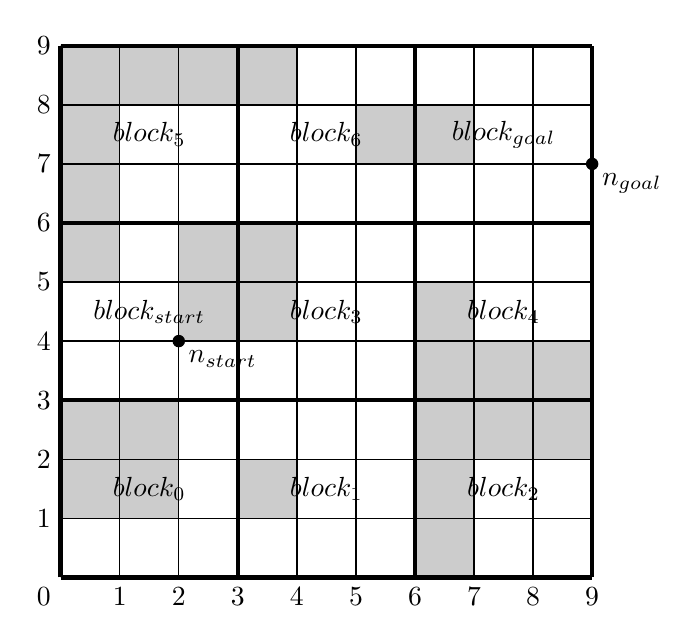
\begin{tikzpicture}[scale=0.75,line width=0.5pt]
    
    \filldraw[black!20] (0,1) rectangle (2,3);
    \filldraw[black!20] (2,4) rectangle (4,6);
    \filldraw[black!20] (0,8) rectangle (4,9);
    \filldraw[black!20] (3,1) rectangle (4,2);
    \filldraw[black!20] (0,5) rectangle (1,8);
    \filldraw[black!20] (6,0) rectangle (7,5);
    \filldraw[black!20] (7,2) rectangle (9,4);
    \filldraw[black!20] (5,7) rectangle (7,8);
    
   \draw[black] (0,0) grid (9,9);

    \node[below left] at (0,0) {0};
    \node[below] at (1,0) {1};
    \node[below] at (2,0) {2};
    \node[below] at (3,0) {3};
    \node[below] at (4,0) {4};
    \node[below] at (5,0) {5};
    \node[below] at (6,0) {6};
    \node[below] at (7,0) {7};
    \node[below] at (8,0) {8};
    \node[below] at (9,0) {9};

    \node[left] at (0,1) {1};
    \node[left] at (0,2) {2};
    \node[left] at (0,3) {3};
    \node[left] at (0,4) {4};
    \node[left] at (0,5) {5};
    \node[left] at (0,6) {6};
    \node[left] at (0,7) {7};
    \node[left] at (0,8) {8};
    \node[left] at (0,9) {9};
    
    \draw[ultra thick] (0,0) -- (9,0);
    \draw[ultra thick] (0,3) -- (9,3);
    \draw[ultra thick] (0,6) -- (9,6);
    \draw[ultra thick] (0,9) -- (9,9);
    \draw[ultra thick] (0,0) -- (0,9);
    \draw[ultra thick] (3,0) -- (3,9);
    \draw[ultra thick] (6,0) -- (6,9);
    \draw[ultra thick] (9,0) -- (9,9);
    
    \node at (1.5,1.5) {$block_{0}$};
    \node at (4.5,1.5) {$block_{1}$};
    \node at (7.5,1.5) {$block_{2}$};
    \node at (1.5,4.5) {$block_{start}$};
    \node at (4.5,4.5) {$block_{3}$};
    \node at (7.5,4.5) {$block_{4}$};
    \node at (1.5,7.5) {$block_{5}$};
    \node at (4.5,7.5) {$block_{6}$};
    \node at (7.5,7.5) {$block_{goal}$};
    
    \fill (2,4) circle (3pt);
    \node[below right] at (2,4) {$n_{start}$};
    \fill (9,7) circle (3pt);
    \node[below right] at (9,7) {$n_{goal}$};

  \end{tikzpicture}
  \end{center}
 
\noindent 
When expanding $block_{4}$:
\begin{description}
\item[$listX$] = \\ \hfill (6,3),(7,3),(8,3),(9,3),(6,4),(6,5),(6,6),(7,6),(8,6),(9,6) from $block_{4}$\\
\item[$listX'$] = \\ \hfill (6,3),(7,3),(8,3),(9,3) from $block_{2}$,\\ (6,3) from $block_{1}$,\\ (6,3),(6,4),(6,5),(6,6) from $block_{3}$,\\ (6,6) from $block_{6}$,\\ (6,6),(7,6),(8,6),(9,6) from $block_{goal}$
\end{description}

  \caption{Block A*: map of {$ 9 \times 9$} cells is split into 9 blocks of {$ 3 \times 3$} cells} 
  \label{fig:lineofsight}
\end{figure}


\clearpage
\section {Requirements analysis}

As specified in the `Work to be done' section of my Proposal (see Appendix E), my project was divided into four sections. This section outlines the functional and non-functional requirements for the system, and their relative priorities using the MoSCoW system. \\
\centerline {{\bf M} - Must; {\bf S} - Should; {\bf C} - Could; {\bf W} - Won't}

\subsection{Testing simulator}

\begin{center}
    \begin{tabular}{ l | p{10cm} | l}
    ID & Functional requirement & Priority  \\ \hline
    1 & The system shall load one of a collection of maps from the generator & M \\ \hline
    2 & The system shall load one of a collection of maps from a saved file & S \\ \hline
    3 & The system shall create a grid-graph from a given map & M \\ \hline
    4 & The system shall create a visibility graph from a given map & C \\ \hline
    5 & The system shall run one of a collection of any-angle path-finding algorithms on a graph and collect data such as the path-length and the length of computation & M \\ \hline
    6 & The system shall display a visual representation of the current map and the paths found by any algorithms that have been run on it & M \\ \hline
    7 & The system shall display the numeric statistics for each path for the current map & M \\ \hline
     \hline 
    ID & Non-functional requirement & Priority  \\ \hline
    1 & The system shall be designed in a modular way to allow easy extension for new algorithms & S \\
    \end{tabular}
\end{center}

\subsection{Map generation}

\begin{center}
    \begin{tabular}{ l | p{10cm} | l }
    ID & Functional requirement & Priority  \\ \hline
    1 & The system shall generate pseudo-random maps of a given resolution, coverage percentage and clustering & M \\ \hline
    2 & The system shall allow maps to be saved so that multiple tests can be run on the same map suite & M \\ \hline
     3 & The system shall allow maps to be created with an interactive map editor & C\\ \hline
          \hline 
    ID & Non-functional requirement & Priority  \\ \hline
    1 & The system shall generate maps of the highest resolution in under 2 seconds & S \\
    \end{tabular}
\end{center}
	
\subsection{Algorithm implementation}

\begin{center}
    \begin{tabular}{ l | p{10cm} | l}
    ID & Functional requirement & Priority  \\ \hline
    1 & The system shall correctly implement each of the chosen algorithms. If a path exists, the path and numerical statistics will be returned. If no path exists, this will be returned   & M \\ \hline
    2 & The system shall allow arbitrary start and end coordinates for any map & S \\ \hline
     \hline 
    ID & Non-functional requirement & Priority  \\ \hline
    1 & The system shall be designed in a modular way to allow easy extension for new algorithms & S \\
    \end{tabular}
\end{center}

\subsection{Data gathering}

\begin{center}
    \begin{tabular}{ l | p{10cm} | l}
    ID & Functional requirement & Priority  \\ \hline
    1 & The system shall write statistics for an arbitrary set of specified algorithms on an arbitrary set of specified maps and write the results to a CSV file & M \\ \hline
     \hline 
    ID & Non-functional requirement & Priority  \\ \hline
    1 & The system shall be designed with a clear API that enables quick and easy data gathering. & M \\
    \end{tabular}
\end{center}

\noindent
To do - use case diagrams etc.

\section {Testing}

To do.

\section {Design model}

\noindent
Having completed the preparation phase of the project, I refined the plan for the implementation phase from that presented in the Project Proposal (see Appendix ?). An incremental model of implementation was adopted, with new modules being developed and tested separately before being integrated into the work program. The milestones of the project were:
\begin{description}
\item {\em Milestone 1} - Maps of arbitrary size, coverage and clustering can be created and printed to system output.
\item {\em Milestone 2} - Arbitrary maps can be converted to grape, and A* can be run on these maps. A visual representation of the path can be printed to system output.
\item {\em Milestone 3} - Basic UI is built, including all functionality from {\em Milestone 2}. Basic path statistics are displayed.
\item {\em Milestone 4} - Map saving, map loading and map creation functionality are present. This will facilitate debugging edge cases for more complex algorithms.
\item {\em Milestone 5} - Line of sight, A* with post-smoothing, $\theta ^{*}$ and Lazy $\theta ^{*}$ are implemented.
\item {\em Milestone 6} - Block A* is implemented.
\item {\em Milestone 7} - Data extraction scripts are implemented.
\end{description}

\section {Languages and tools}

\begin{description}
  \item[Programming language] \hfill \\
  {\em Java} - provides abstraction and class hierarchy to enable development of modular, extensible code.
  \item[Libraries] \hfill \\
  {\em Swing} - for graphical user interface design and {\em CSVWriter} for data export.
  \item[Integrated development environment] \hfill \\
  {\em Eclipse} - allows rapid development through integrated testing, refactoring and version control tools.
  \item[Statistical analysis and visualisation] \hfill \\
  {\em R} - an open-source statistical package, due to its flexibility and extensibility.
  \item[Backup] \hfill \\
  {\em DropBox} and {\em Google Drive} - both of which maintain multiple shadow copies of my work in the cloud.
  \item[Version Control]\hfill \\
  {\em GitHub} - which facilitated exploring different implementation strategies by forking my core code repository.
  
\end{description}

\cleardoublepage
\chapter{Implementation}

In this chapter I will give an overview of the implementation of the project, as well as investigating some of its more interesting features.\\

\noindent
The chapter will be split into six parts: 
\begin{description}
  \item{\bf Map generation}\\ \hfill  an explanation of the algorithm used to generate maps.
  \item{\bf Simulation}\\ \hfill an overview of the simulator, including graph generation and algorithm data.
  \item{\bf Algorithms}\\ \hfill each of the algorithms will be covered, with specific attention given to Block A*.
  \item{\bf User Interface}\\ \hfill an overview of the graphical user interface. 
  \item{\bf Testing}\\ \hfill an overview of the methods used to test the code for correctness.
  \item{\bf Data extraction}\\ \hfill an explanation of how large volumes of data were extracted for statistical analysis.
\end{description}

\begin{figure}
  \centering
  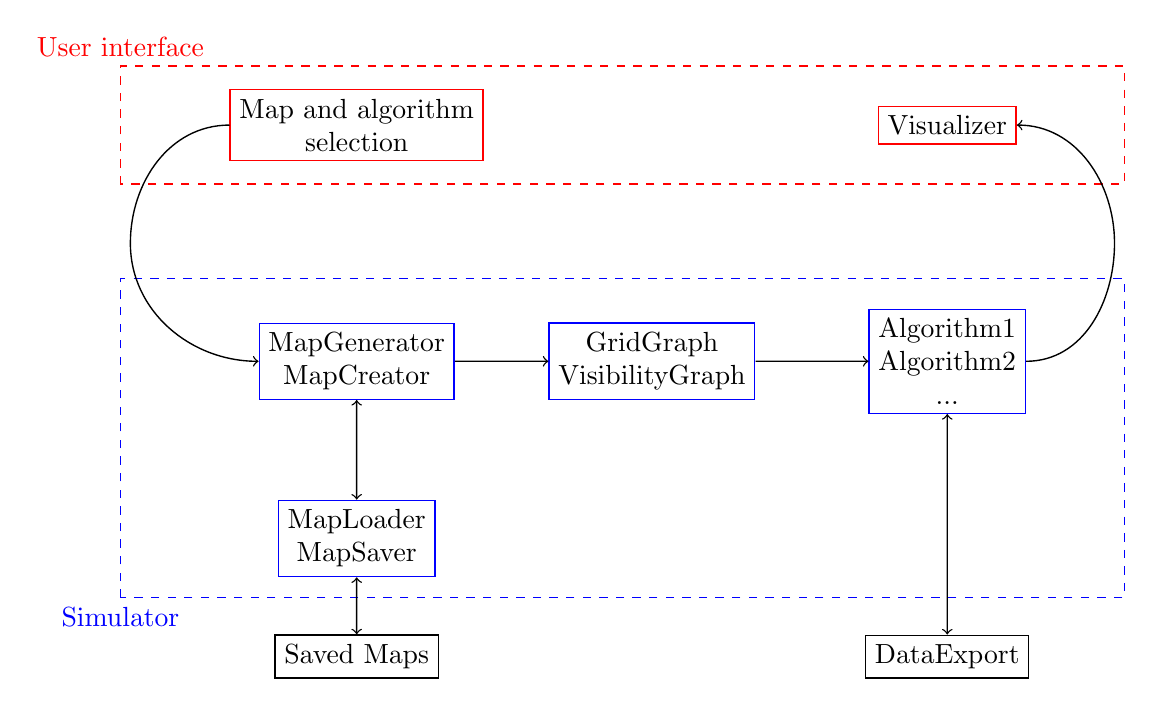
\begin{tikzpicture}[scale=0.75,line width=0.5pt]
  \filldraw[color=red,fill=white,dashed] (0,5) rectangle (17,7); 
  \node[above, red] at (0,7) {User interface};
  \filldraw[color=blue,fill=white,dashed] (0,-2) rectangle (17,3.4); 
  \node[below, blue] at (0,-2) {Simulator};
  
\node[draw=red,shape=rectangle,align=center] at (4,6) (1) {Map and algorithm \\selection};
\node at (0,4) (2) {};
\node[draw=blue,shape=rectangle,align=center] at (4,2) (3) {MapGenerator\\MapCreator};
\node[draw=blue,shape=rectangle,align=center] at (9,2) (4) {GridGraph\\VisibilityGraph};
\node[draw=blue,shape=rectangle,align=center] at (14,2) (5) {Algorithm1\\Algorithm2\\...};
\node at (17,4) (6) {};
\node[draw=red,shape=rectangle,align=center] at (14,6) (7) {Visualizer};
\node[draw=blue,shape=rectangle,align=center] at (4,-1) (8) {MapLoader\\MapSaver};
\node[draw=black,shape=rectangle,align=center] at (4,-3) (9) {Saved Maps};
\node[draw=black,shape=rectangle,align=center] at (14,-3) (10) {DataExport};

\draw[->] (1.west) to[out=180,in=90] (2.east) to[out=-90,in=180] (3.west);
\draw[->] (3) to (4);
\draw[->] (4) to (5);
\draw[->] (5.east) to[out=0,in=-90] (6.west) to[out=90,in=0] (7.east);
\draw[<->] (3) to (8);
\draw[<->] (8) to (9);
\draw[<->] (5) to (10);


  \end{tikzpicture}
  \caption{Flow of the user interface and simulator} 
  \label{fig:lineofsight}
\end{figure}

\newpage
\section{Map generation}

In order to reach reliable conclusions about the performance of the algorithms, I needed a way to generate large volumes of maps of a given resolution $N$, coverage percentage $C$ and clustering $D$. I devised an algorithm to pseudo-randomly create such maps. The algorithm creates maps of varying clustering by loosely approximating the idea of potential fields.\\

\noindent
The input to the algorithm includes an integer matrix $m_{i,j}$ of size $N^{2}$ - where each element has been initialised to value 1. At any point in the algorithm, $m_{i,j}$'s value represents its `potential' - i.e. the chance that $m_{i,j}$ will be the next element set to 0 (i.e. blocked). The algorithm performs $C \times N^{2}$ iterations. In each iteration, it chooses a random number $r$ between $0$ and $\sum\limits_{i,j} m_{i,j}$. It then traverses the matrix row-by-row until the sum of the elements it has seen is at least $r$. The potential of the element that has been reached is set to $0$, and the potential of the surrounding elements is increased in a crude approximation of a potential field. The output is an integer matrix $m_{i,j}$ of size $N^{2}$ - where $C\%$ of the elements have value 0, which denotes a blocked cell, and the rest of the elements have value \textgreater $0$, which denotes a free cell. The array can then be parsed into a {\tt Map} by the {\tt Map} constructor.

\begin{algorithm}[htp]
  \SetAlgoLined\DontPrintSemicolon
  \SetKwFunction{genMap}{GenerateMap} \SetKwFunction{setBlocked}{SetAsBlocked}
  \SetKwProg{myDef}{def}{}{}
  \myDef{\genMap{$m, C, D$}}{
    \nl \Repeat{$(C\times N^{2}) times$} {
      \nl $r \gets random(0,\sum\limits_{i,j} m_{i,j})$\;
      \nl $i,j \gets 0$\;
      \nl \While{$r\geq 0$} {
        \nl $r \gets r - m_{i,j}$\;
        \nl \uIf{$i < R-1$} {
          \nl $i \gets i+1$\;
        } \nl \Else {
          \nl $i \gets 0$\;
          \nl $j \gets j+1$\;
        }
     }
     \nl \setBlocked{$i,j$};     
  }
  }
  \myDef{\setBlocked{$m_{i,j}$}} {
    \nl $m_{i,j} \gets 0$\;
    \nl \ForEach {$m_{k,l}$ in $horizontalOrVerticalNeighbour(m_{i,j})$} {
      \nl \uIf{$m_{k,l} \neq 0$} {
        \nl $m_{k,l} \gets m_{k,l} + D$\;
      }
  }
  \nl \ForEach {$ m_{k,l}$ in  $diagonalNeighbour(m_{i,j})$} {
      \nl \uIf{$m_{k,l} \neq 0$} {
        $m_{k,l} \gets a_{k,l} + 2\times D$\;
      }
  }
}
\caption{{\sc GenerateMap}}
 \end{algorithm} 
 
 \begin{figure}[h]
\begin{subfigure}{.3\textwidth}
    \centering
    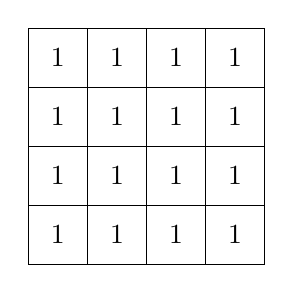
\begin{tikzpicture}[scale=0.75,line width=0.5pt]

     \draw (0,0) grid (4,4);
    
     \foreach \x in {0,1,2,3} {
        \foreach \y in {0,1,2,3} {
          \pgfmathparse{(\x + 0.5)};
          \let\xa\pgfmathresult;
          \pgfmathparse{\y + 0.5};
          \let\ya\pgfmathresult;
          \node at (\xa,\ya) {1};
        }
      }
           
    \end{tikzpicture}
    \caption{Initialisation}
    %\label{fig:sfig1}
  \end{subfigure}
  \begin{subfigure}{.3\textwidth}
    \centering
    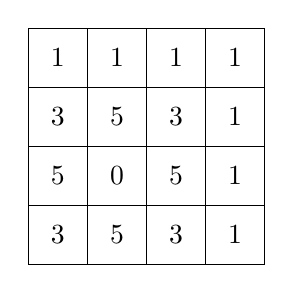
\begin{tikzpicture}[scale=0.75,line width=0.5pt]
     \draw (0,0) grid (4,4);
    
    \node at (0.5,0.5) {3};
    \node at (1.5,0.5) {5};
    \node at (2.5,0.5) {3};
    \node at (3.5,0.5) {1};
    \node at (0.5,1.5) {5};
    \node at (1.5,1.5) {0};
    \node at (2.5,1.5) {5};
    \node at (3.5,1.5) {1};
    \node at (0.5,2.5) {3};
    \node at (1.5,2.5) {5};
    \node at (2.5,2.5) {3};
    \node at (3.5,2.5) {1};
    \node at (0.5,3.5) {1};
    \node at (1.5,3.5) {1};
    \node at (2.5,3.5) {1};
    \node at (3.5,3.5) {1};
      
    \end{tikzpicture}
    \caption{Iteration 1: r = 5}
    %\label{fig:sfig1}
  \end{subfigure}
  %
  \begin{subfigure}{.3\textwidth}
    \centering
    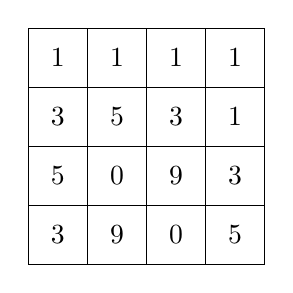
\begin{tikzpicture}[scale=0.75,line width=0.5pt]
    
    \draw (0,0) grid (4,4);
    
    \node at (0.5,0.5) {3};
    \node at (1.5,0.5) {9};
    \node at (2.5,0.5) {0};
    \node at (3.5,0.5) {5};
    \node at (0.5,1.5) {5};
    \node at (1.5,1.5) {0};
    \node at (2.5,1.5) {9};
    \node at (3.5,1.5) {3};
    \node at (0.5,2.5) {3};
    \node at (1.5,2.5) {5};
    \node at (2.5,2.5) {3};
    \node at (3.5,2.5) {1};
    \node at (0.5,3.5) {1};
    \node at (1.5,3.5) {1};
    \node at (2.5,3.5) {1};
    \node at (3.5,3.5) {1};
      
    \end{tikzpicture}
    \caption{Iteration 2: r = 2}
    %\label{fig:sfi2}
  \end{subfigure}
  \caption{Two iterations of {\tt GenerateMap} with $R$=4 and $D$=2}
  %\label{fig:fig}
\end{figure}

\newpage
\section{Simulation}

\subsection{Graph Generation}

To create a graph from a map, the map was iterated over twice. The first iteration created nodes for all the coordinates that were valid node locations. The second iteration set the neighbours of each node. Checks for both of the iterations were performed by checking whether neighbouring blocks were blocked. See Figure 3.3.\\

\begin{figure}
\begin{lstlisting}
...
Coordinate[] diagonalRelativeCellCoordinates = 
		{new Coordinate(-1,-1), new Coordinate(0,-1), 
		new Coordinate(0,0), new Coordinate(-1,0)};
		
Node[][] graphArray2D = 
	new Node[map.getWidth()+1][map.getHeight()+1];
for(int j=0; j < map.getHeight()+1; j++) {
	for(int i=0; i < map.getWidth()+1; i++) {
		boolean isUnblockedAdjacentCell = false;
		for(Coordinate c: diagonalRelativeCellCoordinates) {
			try {
				if(!map.getCell(i+c.getX(),j+c.getY()).isBlocked()) {
					isUnblockedAdjacentCell=true;
				}
			} catch (ArrayIndexOutOfBoundsException e) {}
		}
		if(!isUnblockedAdjacentCell) {
			graphArray2D[i][j] = null;
		} else {
			graphArray2D[i][j] = new Node(new Coordinate(i,j));
		}
	}
}
...
\end{lstlisting}
\caption{Code snippet showing {\tt Node} creation for grid-based graphs}
\end{figure}

\noindent
As discussed in the Preparation chapter, along with grid-based graphs, I am also going to investigate the performance benefits of running path-finding algorithms on visibility graphs. The creation of visibility graphs depends on having a {\tt LineOfSight} function.\\

\noindent
{\bf Line of Sight}\\

\noindent
The line of sight algorithm is based on the pseudocode in [reference Theta* paper], which itself is a derivative of Bresenham's line drawing algorithm - though instead of choosing pixels (i.e. cells) to draw, it chooses cells to check whether they are blocked. Bresenham's algorithm is a useful framework as it avoids any floating point calculations when the start and end points are integers - this has dual benefits:
\begin{itemize}
\item the algorithm is fast
\item the algorithm doesn't suffer from rounding errors inherent in floating-point calculations. 
\end{itemize}
\noindent
A notable alteration to the basic Bresenham algorithm is that instead of checking one cell per column (or one per row), the line of sight algorithm will check any cell that the real line passes through. This only requires a minor alteration.\\

\noindent
For the purposes of clarity, the pseudocode presented in {\sc LineOfSight} assumes the line of sight is in octant 1 - i.e. whose angle with the x-axis is between $0^{o}$ and $45^{o}$. The full pseudocode can be found in Appendix ?. On this assumption, the key variables are:
\begin{description}
\item{$x$ and $y$} - integers that represent the coordinate of the cell being considered, which is always a cell that the line passes through.
\item{$f$} - a value that represents at what point the line intersects $x+1$ with respect to the current $y$ value. See Figure 3.4.
\end{description}

\noindent
The algorithm starts at $n_{start}$. The current f-value is increased by $dy$ every time $x$ is increased, but decreased by $dx$ if $y$ is increased. If at any point $f = 0$ then the line intersects the bottom right-corner of the cell currently being considered, or if $y = dy$ then it intersects at the top left-corner. Therefore, if $f > 0$ then we need to check the $cell_{x,y}$ to see if it's blocked and if $f > dy$ then we additionally need to check $cell_{x,y+1}$.\\

\noindent
{\em Note:} to disallow a line of sight through a `diagonal blockage' (as introduced in section 2.1.3, a new {\bf if} clause would be added after line 18 of {\sc LineOfSight}:\\
\noindent 
{\tt {\bf if} $f = 0 \land cell_{x,y}.isBlocked() \land cell_{x+1,y-1}.isBlocked()$ {\bf then return} $false$}.\\
\noindent 
To avoid the possibility of the final clause in the condition throwing an {\tt ArrayIndexOutOfBoundsException}, an extra $x$-coordinate check or a {\tt try-catch} block would also be required.

\begin{figure}[h]
\centering
  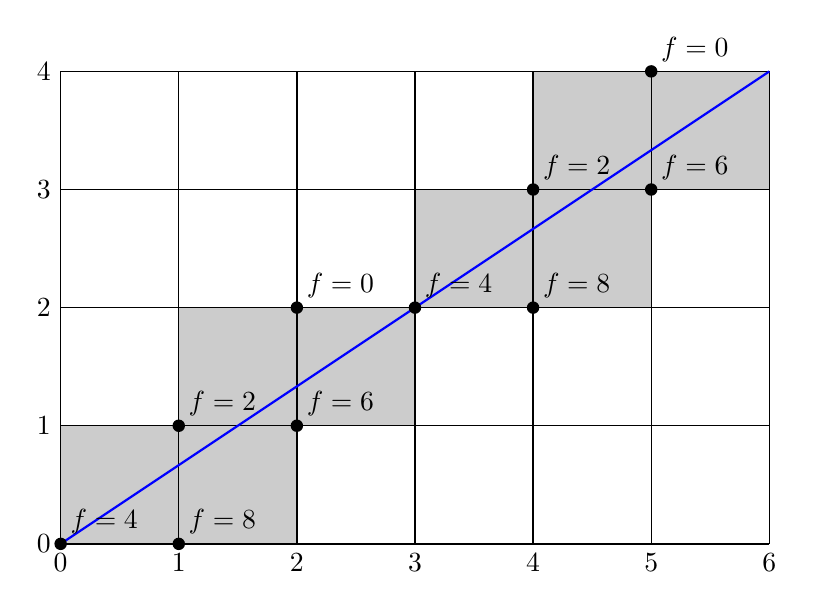
\begin{tikzpicture}[scale=1.5,line width=0.5pt]
    \draw (0,0) grid (6,4);

    \node[below] at (0,0) {0};
    \node[below] at (1,0) {1};
    \node[below] at (2,0) {2};
    \node[below] at (3,0) {3};
    \node[below] at (4,0) {4};
    \node[below] at (5,0) {5};
    \node[below] at (6,0) {6};

    \node[left] at (0,0) {0};
    \node[left] at (0,1) {1};
    \node[left] at (0,2) {2};
    \node[left] at (0,3) {3};
    \node[left] at (0,4) {4};

    \filldraw[color=black,fill=black!20] (0,0) rectangle (1,1); 
    \filldraw[color=black,fill=black!20] (1,0) rectangle (2,1);
    \filldraw[color=black,fill=black!20] (1,1) rectangle (2,2);
    \filldraw[color=black,fill=black!20] (2,1) rectangle (3,2);
    \filldraw[color=black,fill=black!20] (3,2) rectangle (4,3); 
    \filldraw[color=black,fill=black!20] (4,2) rectangle (5,3);
    \filldraw[color=black,fill=black!20] (4,3) rectangle (5,4);
    \filldraw[color=black,fill=black!20] (5,3) rectangle (6,4);
    
    \draw[blue, thick] (0,0) -- (6,4);
  
    \node[above right] at (0,0) {$f=4$}; \fill (0,0) circle (1.5pt);
    \node[above right] at (1,0) {$f=8$}; \fill (1,0) circle (1.5pt);
    \node[above right] at (1,1) {$f=2$}; \fill (1,1) circle (1.5pt);
    \node[above right] at (2,1) {$f=6$}; \fill (2,1) circle (1.5pt);
    \node[above right] at (2,2) {$f=0$}; \fill (2,2) circle (1.5pt);
    \node[above right] at (3,2) {$f=4$}; \fill (3,2) circle (1.5pt);
    \node[above right] at (4,2) {$f=8$}; \fill (4,2) circle (1.5pt);
    \node[above right] at (4,3) {$f=2$}; \fill (4,3) circle (1.5pt);
    \node[above right] at (5,3) {$f=6$}; \fill (5,3) circle (1.5pt);
    \node[above right] at (5,4) {$f=0$}; \fill (5,4) circle (1.5pt);

  \end{tikzpicture}
  \caption{Line of sight algorithm} \label{fig:lineofsight}
\end{figure}

\begin{algorithm}[htp]
  \SetAlgoLined\DontPrintSemicolon
  \SetKwFunction{los}{LineOfSight}
  \SetKwProg{myDef}{def}{}{}
  \myDef{\los($n_{source}$,$n_{goal}$)}{
    \nl $ x \gets n_{source}.x$\;
    \nl $ y \gets n_{source}.y$\;
    \nl $ x_{goal} \gets n_{goal}.x$\;
    \nl $ y_{goal} \gets n_{goal}.y$\;
    \nl $ dx \gets x_{goal} - x$\;
    \nl $ dy \gets y_{goal} - y$\;
    \nl $ f \gets 0$\;
    \nl \While{$x \neq x_{goal}$} {
      \nl $f \gets f + dy$\;
      \nl \uIf{$x \geq dx$} {
        \nl \uIf{$cell_{x,y}.isBlocked()$} {
          \nl \KwRet{$false$}\;
        }
        \nl $y \gets y+1$\;
        \nl $f \gets f - 1$\;
      }
      \nl \uIf{$f \neq 0 \land cell_{x,y}.isBlocked()$} {
        \nl \KwRet{$false$}\;
      }
      \nl \uIf{$dy = 0 \land cell_{x,y}.isBlocked() \land cell_{x,y-1}.isBlocked()$} {
        \nl \KwRet{$false$}\;
      }
      \nl $x \gets x + 1$\;
    }
    \nl \KwRet{$true$}\;
  }
  \caption{{\sc LineOfSight}}
\end{algorithm} 

\subsection{Algorithm Data}

Each {\tt MapInstance} has a {\tt Map}, a {\tt Graph} and an {\tt AlgorithmData} object for each of the algorithms that have been run on that map.\\

\begin{figure}
\centering
\begin{tikzpicture} 
\umlsimpleclass{MapInstance} 
\umlsimpleclass[x=-4,y=-2.5]{Map} 
\umlsimpleclass[x=0,y=-2.5]{Graph}
\umlsimpleclass[x=4,y=-2.5,type=abstract]{AlgorithmData}
\umlsimpleclass[x=-4,y=-5]{Cell} 
\umlsimpleclass[x=0,y=-5]{Node} 
%\umlclass[x=4,y=-3,type=abstract]{AlgorithmData}{- distance : $double$ \\ - angle : $double$ \\ - path : $List<Coordinate>$ \\ ...}{+ go() : void \\ \# getPath($graph : Graph$) : $Node$ \\ ...} 
\umlHVuniassoc[arg1=1, pos1=0.2, align1=left,arg2=1, pos2=2, align2=right]{MapInstance}{Map}
\umluniassoc[arg1=1, pos1=0.3, align1=right,arg2=1, pos2=1, align2=right]{MapInstance}{Graph}
\umlHVuniassoc[arg1=1, pos1=0.2, align1=right, arg2=6, pos2=2, align2=right]{MapInstance}{AlgorithmData}
\umluniassoc[arg1=1, pos1=0.3, align1=right,arg2=*, pos2=1, align2=right]{Map}{Cell}
\umluniassoc[arg1=1, pos1=0.3, align1=right,arg2=*, pos2=1, align2=right]{Graph}{Node}
\umluniassoc[mult1=1,pos1=0,mult2=*,pos2=1, angle1=-45, angle2=-135, loopsize=3cm]{Node}{Node}
\end{tikzpicture}
\caption{Composition of {\tt MapInstance}}
\end{figure}

\noindent
{\tt AlgorithmData} is an abstract class to facilitate adding new algorithms in a modular way. It has a public method {\tt go()}, as well as getter methods for all statistical data about each algorithm. {\tt go()} calls the $getPath(n_{start},n_{goal})$ method, which returns $n_{goal}$ if a path is found, or $null$ otherwise. If $null$ is returned, this is recorded in the statistics. If $n_{goal}$ is returned, {\tt go()} calculates some of the statistics as follows:

\begin{description}
\item {\bf Path length}\\ \hfill
the sum of the Euclidean distances between each pair of consecutive nodes in the path.
\item {\bf Cumulative path angle}\\ \hfill
the sum of the scalar product between each pair of adjacent path segments in the path.
\item {\bf Graph calculation time}\\ \hfill
{\tt System.nanoTime()} is used to calculate the duration between the call to {\tt generateGraph()} and it returning.
\item {\bf Path calculation time}\\ \hfill
{\tt System.nanoTime()} is used to calculate the duration between the call to {\tt getPath()} and it returning.
\item {\bf Number of nodes expanded}\\ \hfill
a counter was incremented each time a node was expanded. It should be noted that in Block A*, node expansion is not the same as block expansion.
\end{description}

\section{Algorithms}

To emphasise the close relationships between the algorithms and allow for maximum code re-use, I organised the concrete instances of {\tt AlgorithmData} in a hierarchy. This also ensured that any performance differences between algorithms was due to the different nature of each algorithm and not different implementation of similar concepts. See Figure 3.5.\\

\begin{figure}
\centering
\begin{tikzpicture} 
\umlemptyclass[type=abstract]{AlgorithmData}
\umlemptyclass[x=-2,y=-3]{Dijkstra}
\umlemptyclass[x=2,y=-3]{BlockAStar}
\umlemptyclass[x=-2,y=-6]{AStar}
\umlemptyclass[x=-2,y=-9]{AStarSmoothed}
\umlemptyclass[x=2,y=-9]{ThetaStar}
\umlemptyclass[x=2,y=-12]{LazyThetaStar}
\umlVHVreal{Dijkstra}{AlgorithmData}
\umlVHVreal{BlockAStar}{AlgorithmData}
\umlVHVinherit{AStar}{Dijkstra}
\umlVHVinherit{AStarSmoothed}{AStar}
\umlVHVinherit{ThetaStar}{AStar}
\umlVHVinherit{LazyThetaStar}{ThetaStar}

\end{tikzpicture}
\caption{Inheritance structure of algorithms}
\end{figure}

\subsection{Dijkstra's shortest paths}

The implementation was based on the pseudo-code seen in section 2.2.1. Details of note include:
\begin{description}
  \item {\bf Open Set}\\ \hfill
  the standard {\tt java.util.PriorityQueue} would occasionally not return the node with the smallest g-value when $openSet.pop()$ was called. This is a documented bug for large queues that occurs when a queue item has its priority\footnote{In this case, the {\tt Node}'s g-value} altered while residing in the $openSet$, so l had to manually $pop()$, $update()$ and re-$add()$ any node that needed to be updated when already in the $openSet$.
  \item {\bf Closed set}\\ \hfill
  the only two operations on the {\tt closedSet} are adding and checking for membership. Therefore, a {\tt HashSet} was used for its average case O(1) insertion and search speed.
  \item {\bf Extensibility} \\ \hfill
  to allow a clear algorithm hierarchy, I needed to add a call to $initialise(n)$ whenever a node $n$ was popped from the $openSet$, and a $postProcessing(n)$ step before the node is returned. In {\tt Dijkstra} these have empty method bodies, but some of the algorithms that inherit from Dijkstra will override these methods.
  \end{description}


\subsection{A*}

The implementation was based on the pseudo-code seen in section 2.2.2: A* inherits from Dijkstra, and overrides the $updateCost()$ function.

\subsection{A* with post-smoothing}

The implementation was based on the pseudo-code seen in section 2.2.3: A* inherits from A* with post-smoothing and implements its post-smoothing by overriding the $postProcessing()$ function.\\

\subsection {Basic $\theta ^{*}$ and Lazy $\theta ^{*}$}

The implementation was based on the pseudo-code seen in section 2.2.4 and 2.2.5: 
\begin{description}
\item{\bf Basic $\theta ^{*}$}\\ \hfill inherits from A*, and overrides the $updateCost()$ function
\item {\bf Lazy $\theta ^{*}$ }\\ \hfill inherits from Basic $\theta ^{*}$, and overrides the $initialiseNode()$ and $updateCost()$ functions
\end{description}

\subsection {Block A*}

{\bf Local Distance Database}\\

\noindent
The first challenge was to obtain an LDDB. Since there was no publicly available library containing the LDDBs, I had to create my own. Although it would have been possible to create the entries manually for the LDDB for block sizes of $2 \times 2$ cells, this would certainly not have been feasible for block sizes that were any larger, since for blocks of size {$n \times n$}, there will be $2^{n^{2}}$ possible blocks, each with $4.n.4.(n-1)$ pairs of ingress and egress coordinates, which gives over 12 million calculations for a block size of $4 \times 4$.\\

\noindent
I calculated the shortest paths using A* over visibility graphs, which gives provably optimal paths.\\

\noindent
For a given block size , I required:\\
\indent for every possible block of size {$n \times n$}\\
\indent \indent for every possible ingress-egress coordinate pair\\
\indent \indent \indent (a) the shortest path between that pair\\
\indent \indent \indent (b) a list containing every intermediate coordinate on that path.\\

\noindent
It was necessary to put these entries into a database structure that would be compact in memory and fast to load and query. Since these constraints were fundamental to the operation of the algorithm, any library or 3$^{rd}$ party database implementation could not be guaranteed to be sufficiently specialised for the task, so I implemented my own database using arrays and hash tables to ensure optimal performance and minimum space wastage.\\

\noindent
All queries to the database would need to identify a block and pair of coordinates as an input, and would receive either the length of the shortest path between those nodes, or a list of the intermediate nodes on the shortest path between those two nodes. I devised a simple bitwise encoding scheme to represent blocks as integers that would be much more space and time efficient than storing {\tt Map} objects in the database to use as comparison: each cell in the block is represented by a bit in the integer, and that bit is set if the corresponding cell is blocked. The 32 bits of the integer are sufficient for all the block sizes that are worth considering: $2 \times 2$ to $4 \times 4$.\footnotemark[1]\\

\noindent
Using this scheme, the underlying implementation of my database was an array of {\tt  HashMaps} - one {\tt HashMap} per block, with the array indexed by the code of the block. The {\tt HashMap} mapped a key: a {\tt Pair} of ingress-egress {\tt Coordinate}s, to a value: a {\tt Pair} consisting of the length (as a {\tt double}) of the shortest path and an {\tt ArrayList} of the {\tt Coordinate}s on the path.\\

\begin{figure}
    \centering
    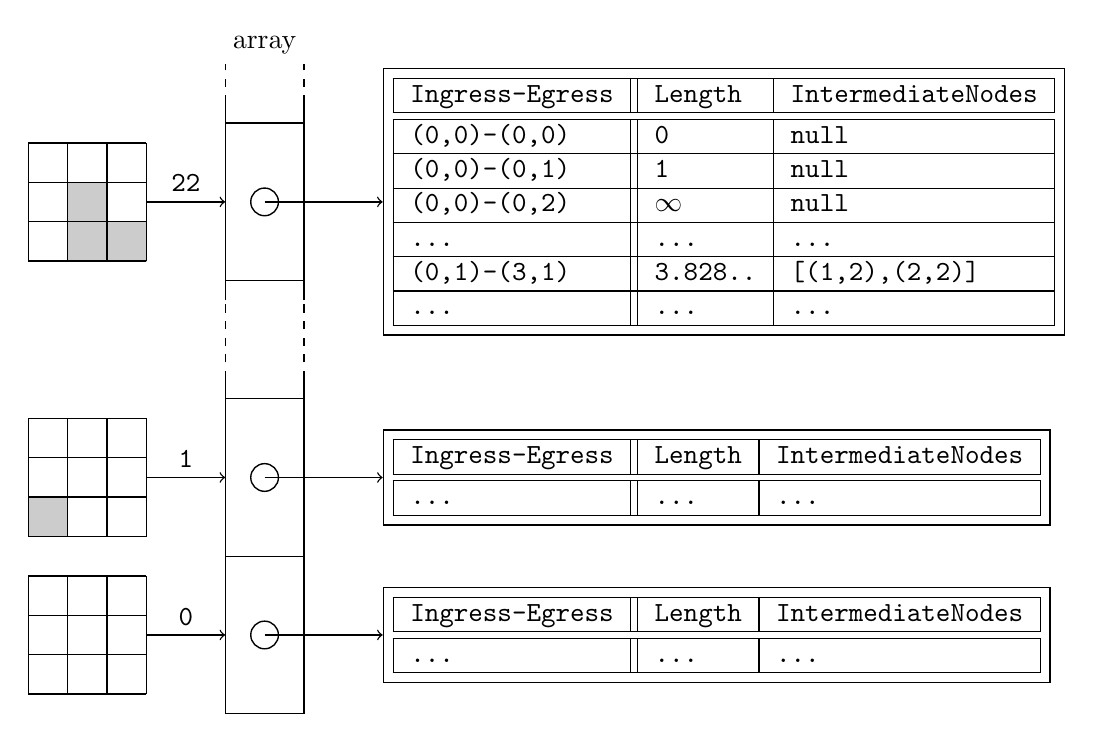
\begin{tikzpicture}[scale=0.5,line width=0.5pt]
    
    \filldraw[black!20] (0,4) rectangle (1,5);
    
    \filldraw[black!20] (1,11) rectangle (2,13);
    \filldraw[black!20] (2,11) rectangle (3,12);
    
      \draw (0,0) grid (3,3);
      \draw (0,4) grid (3,7);
      \draw (0,11) grid (3,14);
      
      \draw (5,-0.5) -- (5,8);
      \draw[dashed] (5,8) -- (5,10);
      \draw(5,10) -- (5,15);
      \draw[dashed] (5,15) -- (5,16);
      \draw (7,-0.5) -- (7,8);
      \draw[dashed] (7,8) -- (7,10);
      \draw(7,10) -- (7,15);
      \draw[dashed] (7,15) -- (7,16);
      
      \draw (5,-0.5) -- (7,-0.5);
      \draw (5,3.5) -- (7,3.5);
      \draw (5,7.5) -- (7,7.5);
      \draw (5,10.5) -- (7,10.5);
      \draw (5,14.5) -- (7,14.5);
      
      \draw[->] (3,1.5) -- (5,1.5);
      \draw[->] (3,5.5) -- (5,5.5);
      \draw[->] (3,12.5) -- (5,12.5);
      
      \node[above] at (4,1.5) {\tt 0};
      \node[above] at (4,5.5) {\tt 1};
      \node[above] at (4,12.5) {\tt 22};
      \node[above] at (6,16) {array};
      
      \draw[->] (6,1.5) -- (9,1.5);   
      \draw (6,1.5) circle (10pt);
      \node[right,draw=black,shape=rectangle] at (9,1.5) (1) {
      \begin{tabular}{| l || l | l |}
    \hline
    {\tt Ingress-Egress} & {\tt Length} & {\tt IntermediateNodes}  \\ \hline \hline
    {\tt ...}  & {\tt ...} & {\tt ...} \\ \hline
    \end{tabular}};
      \draw[->] (6,5.5) -- (9,5.5);
      \draw (6,5.5) circle (10pt);
      \node[right,draw=black,shape=rectangle] at (9,5.5) (1) {
            \begin{tabular}{| l || l | l |}
    \hline
    {\tt Ingress-Egress} & {\tt Length} & {\tt IntermediateNodes}  \\ \hline \hline
    {\tt ...}  & {\tt ...} & {\tt ...} \\ \hline
    \end{tabular}};
      \draw[->] (6,12.5) -- (9,12.5);
      \draw (6,12.5) circle (10pt);
      \node[right,draw=black,shape=rectangle] at (9,12.5) (1) {
    \begin{tabular}{| l || l | l |}
    \hline
    {\tt Ingress-Egress} & {\tt Length} & {\tt IntermediateNodes}  \\ \hline \hline
    {\tt (0,0)-(0,0)}  & {\tt 0} & {\tt null} \\ \hline
    {\tt (0,0)-(0,1)}  & {\tt 1} & {\tt null} \\ \hline
    {\tt (0,0)-(0,2)}  & {\tt $\infty$} & {\tt null} \\ \hline
    {\tt ...}  & {\tt ...} & {\tt ...} \\ \hline
    {\tt (0,1)-(3,1)}  & {\tt 3.828..} & {\tt [(1,2),(2,2)]} \\ \hline
    {\tt ...}  & {\tt ...} & {\tt ...} \\ \hline
\end{tabular}};
      

    \end{tikzpicture}
  \caption{Extract of the LDDB for block size of $3 \times 3$ - array of {\tt HashTable<PairOfCoords,Pair<double,List<Coord>>}s}
  %\label{fig:fig}
\end{figure}

\noindent
This implementation was sufficient but unsatisfactory, as the database sizes were unnecessarily large. This would cause slow loading to memory, less of the LDDB stored in cache and more likelihood of thrashing. Therefore, I compressed the database using bitwise encoding schemes:
\begin{itemize}
\item each {\tt Pair} of ingress-egress {\tt Coordinate}s can be represented with a unique integer representable in a {\tt byte}'s worth of space - so a coding scheme was devised to create an efficient hash function for the {\tt PairOfCoordinate} class.
\item the {\tt List} of intermediate {\tt Coordinate}s can be represented by a code that fits into the 32 bits of an integer: since the maximum number of intermediate nodes on a shortest path in a sub map of size up to {$4 \times 4$} is four\footnotemark[2], and the range of $x$ and $y$ in the {\tt Coordinate} is 0-4, therefore 6 bits can be used for each {\tt Coordinate} - 3 for $x$, 3 for $y$, which is a maximum total of 24 bits.
\end{itemize}

\begin{figure}
\begin{lstlisting}
PairOfCoords(Coordinate c1, Coordinate c2, int blockSize) {
		this.blockSize = blockSize;
		this.coordCode = (byte) 
			(c1.getX() + 
			c1.getY() * (blockSize+1) + 
			c2.getX() * (blockSize+1)*(blockSize+1) + 
			c2.getY() * (blockSize+1)*(blockSize+1)*(blockSize+1));
	}
\end{lstlisting}
\caption{Encoding scheme for {\tt PairOfCoords} in the compressed LDDB}
\end{figure}

\begin{figure}
\begin{lstlisting}
int getListCode(List<Coordinate> intermediateNodes) {
		int listCode = 0;
		for(Coordinate c : intermediateNodes) {
			listCode = listCode | c.getX();
			listCode = listCode << 3;
			listCode = listCode | c.getY();
			listCode = listCode << 3;
		}
		listCode = listCode >>> 3;	//undoes line 7 on final loop
		return listCode;
	}
\end{lstlisting}
\caption{Encoding scheme for {\tt List<Coordinate>} in the compressed LDDB}
\end{figure}

\noindent
These compression techniques allowed me to reduce the size of the databases by about 50\%:

\begin{center}
    \begin{tabular}{| l | l | l |}
    \hline
    Submap size & Size of uncompressed LDDB & Size of compressed LDDB\footnotemark[3]$^{,}$\footnotemark[4]  \\ \hline
    {$2 \times 2$}  & 33KB  & 17KB \\ \hline
    {$3 \times 3$}  & 2.2MB & 1.1MB \\ \hline
    {$4 \times 4$}  & 485MB & 192MB \\ \hline
  \end{tabular}
\end{center}

\noindent
I will investigate the performance of the uncompressed and compressed LDDBs in the Evaluation section.\\
\\

\footnotetext[1]{The exponential increase in size of LDDB would mean that the LDDB for block sizes of $5 \times 5$ or larger take so long to search that performance benefit diminishes.}
\footnotetext[2]{Obtained by experimental results.}
\footnotetext[3]{These savings could be improved further for sub maps of size {$2 \times 2$} and {$3 \times 3$} by using specific data-types depending on the submap size, but this was unnecessary, as the LDDB size was very small compared to the total available memory for sub maps of size{$2 \times 2$} and {$3 \times 3$}, and the LDDB only needs to be loaded into memory once per run of the program.}
\footnotetext[4]{These sizes were significantly larger than those found in Yapp's paper, but his agents were only allowed to travel horizontally and vertically, so only 4 bits were needed to store the path length value.}

\noindent
{\bf Special case blocks: $block_{start}$ and $block_{goal}$} \\

\noindent
$block_{start}$ and $block_{goal}$ are treated as special cases by Block A*. On initialisation:
\begin{itemize}
\item the {\em g-values} of the boundary nodes of $block_{start}$ are set by manually computing shortest paths from $n_{start}$ to each boundary node, instead of looking them up in the LDDB as with other blocks. This is because $n_{start}$ is not guaranteed to be on the boundary of a block, and the LDDB only holds details for routes between boundary nodes
\item the {\em h-values} of the boundary nodes of $block_{goal}$ are set manually for similar reasons.
\item a check is made as to whether $n_{start}$ and $n_{goal}$ are in the same block - i.e. $block_{start}$ equals $block_{goal}$. If so, the shortest path between the two is computed  manually.
\end{itemize}

\noindent
To compute these values, I created a visibility graph for the relevant block and computed the shortest path to each boundary node. Having run some preliminary tests, it became clear that on small maps these initialisations took up to 50\% of the run-time of the algorithm [insert some statistics of test runs]. Therefore, I decided to implement two alternative, extended forms of the LDDB:
\begin{description}
\item{\bf Semi-extended} contains details of shortest paths from {\em any} node to {\em any boundary} node in a block.
\item{\bf Fully-extended} contains details of shortest paths from {\em any} node to {\em any} node in a block.
\end{description}

\noindent
The increase in the size of the LDDB in comparison to the original is:
\begin{center}
    \begin{tabular}{| l | l | l |}
    \hline
    Submap size & Semi-extended & Fully-extended  \\ \hline
    {$2 \times 2$}  & 12.5\% & 26.5\% \\ \hline
    {$3 \times 3$}  & 33.3\% & 77.8\%\\ \hline
    {$4 \times 4$}  & 56.3\% & 144.1\% \\ \hline
  \end{tabular}
\end{center}

\noindent
The use of the fully-extended LDDB allows the initialisation of $block_{start}$ and $block_{goal}$ and the $block_{start}$ equals $block_{goal}$ case to use the LDDB, whereas using semi-extended LDDB requires that the $block_{start}$ equals $block_{goal}$ case finds the shortest route manually.\footnotemark[1] The performance benefits of these different forms of the LDDB will be investigated in the Evaluation chapter.\\

\footnotetext[1]{Note that when using the semi-extended LDDB, $block_{goal}$ needs to reverse the ingress-egress coordinates before querying the LDDB.}

\noindent
{\bf Block A* - algorithm} \\

\noindent
The core of the algorithm was a straightforward implementation, once the details of it were understood. The most challenging part of the implementation was the traceback stage, which was unspecified in the paper. The traceback stage extracts the coordinates of the path from the Graph structure. This requires finding and inserting into a list:
\begin{itemize}
\item the optimal path from $n_{goal}$ to the optimal ingress node of $block_{goal}$
\item the nodes on the optimal path that share block boundaries
\item the intermediate nodes where the optimal path traverses a block
\item the optimal route from the optimal egress node of $block_{start}$ to $n_{start}$
\end{itemize}
\noindent
whilst omitting from the list:
\begin{itemize}
\item all but one of any nodes in this path that lie in the same physical location but belong to different blocks: this occurs when the path crosses block boundaries.
\end{itemize}
 
\section{User Interface}

The user interface was built using Java's Swing toolkit. The UI allows the user to:
\begin{description}
\item{\bf Generate a map} of a given resolution, coverage percentage and clustering.
\item{\bf Create a map} of a given resolution using an interactive editor that has brushes and erasers of differing sizes. If the UI is in map creation mode then UI uses {\tt MouseListener}s to detect when the mouse is being dragged over the map. The array that represents the map is updated according to the size of the brush and the resolution of the map, and then the {\tt repaint()} method of the {\tt JPanel} is called. Once the creation is complete, the array is passed as a parameter to a {\tt Map} constructor, and the {\tt Map} object is passed to the Simulator.
\item{\bf Save a map} with or without paths and statistics.
\item{\bf Load a map} with or without paths and statistics.
\item{\bf Choose start and end points} for the paths on the current map. If the UI is not in map creation mode then {\tt MouseListener}s are used to detect where on the screen the mouse is clicked. The start and end points can be set anywhere on the map.
\item{\bf Calculate paths} for each of the 6 algorithms on the current map. If there is no path then {\tt NoPath} will be displayed.
\item{\bf Display paths} once the path has been calculated
\end{description}

\begin{figure}
\centering
\shadowpicture{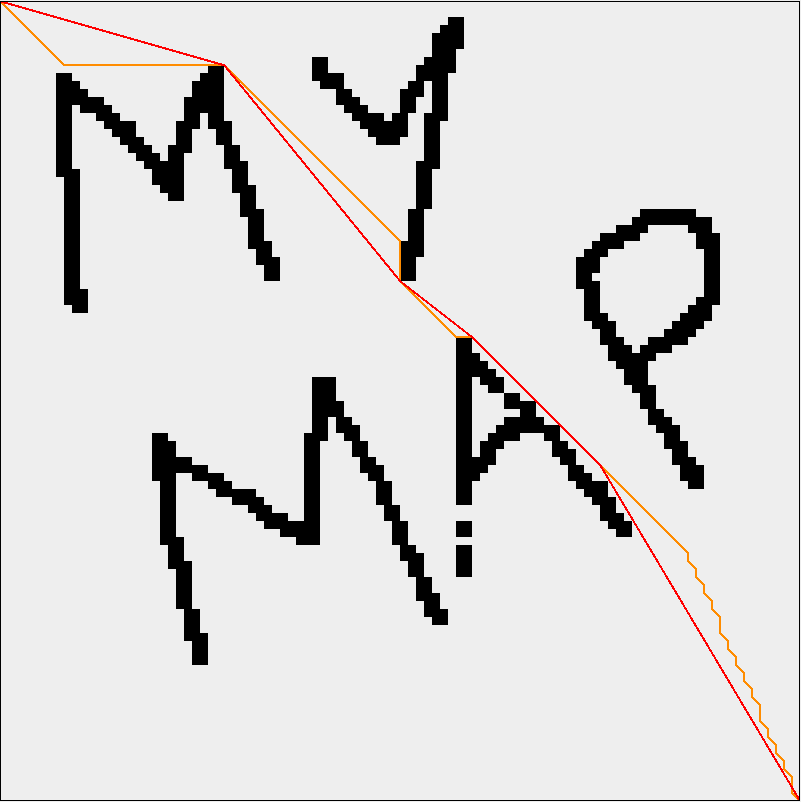
\includegraphics[width=0.8\textwidth]{creationmode.png}}
\caption{User interface in map creation mode}
\end{figure}

\begin{figure}
\centering
\shadowpicture{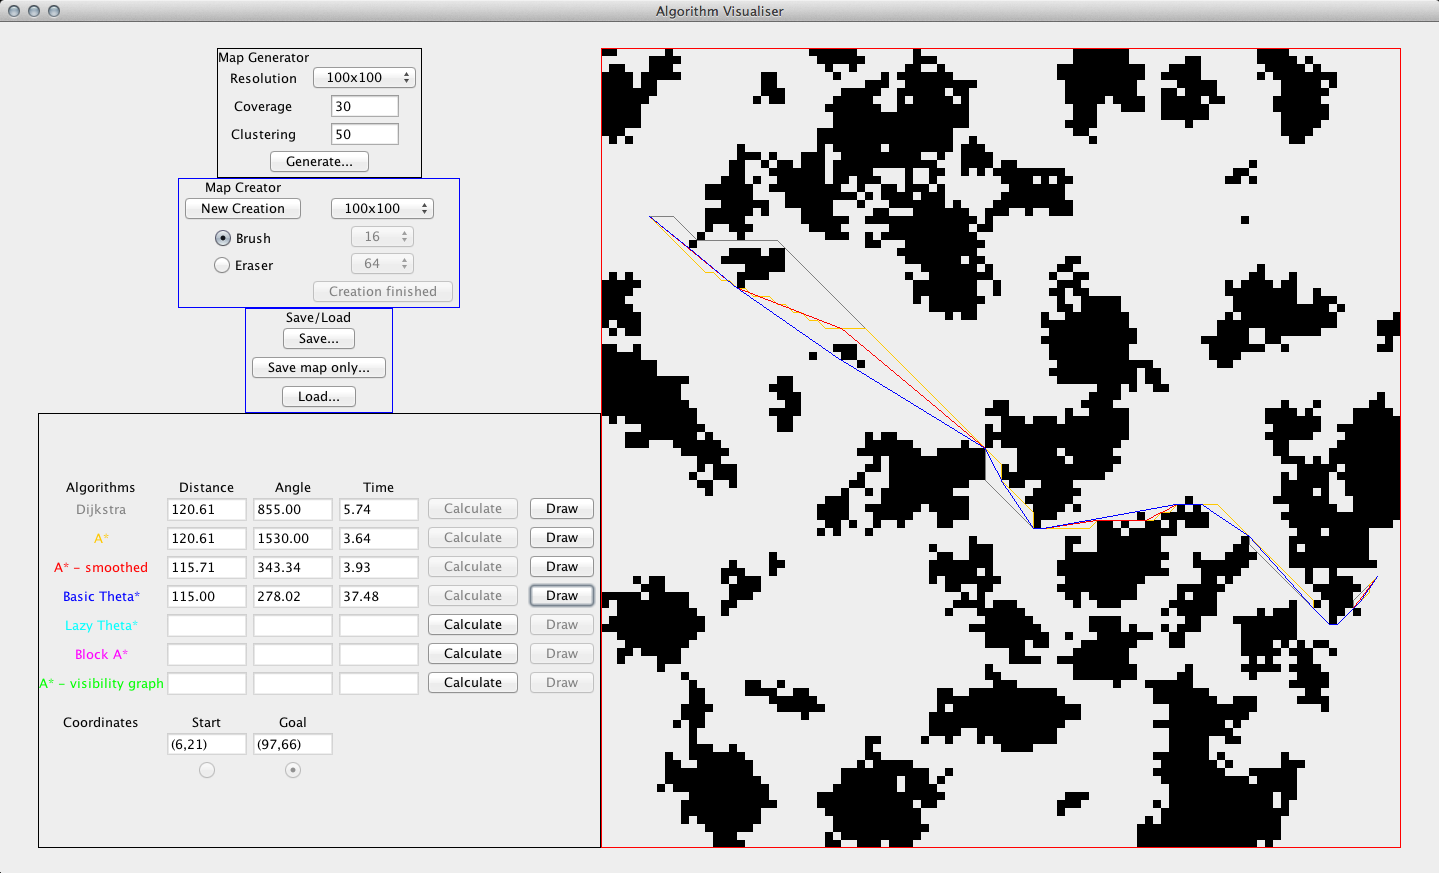
\includegraphics[width=0.8\textwidth]{paths.png}}
\caption{User interface displaying paths for a generated map}
\end{figure}

\section{Testing}

To do.

\section{Data extraction}

To harvest enough data to do meaningful statistical analysis of the performance of the algorithms, the simulator was designed to have a simple API that allowed both a UI to be bolted on and scripts that could bypass the UI altogether. I used the open source package {\tt CSVWriter} to write the data obtained to CSV files, as these are the standard input for $R$ based statistical analysis.

\begin{figure}
\centering
    \begin{tabular}{| l | l | l | l | l |}
    \hline
    Map & Algorithm & PathTime & TotalLength & TotalAngle\\ \hline % & NodesExp\\ \hline
     Map 1 & Dijkstra & 852.926976 & 160.752308679 & 495.0000736525\\ \hline % & 8203\\ \hline
     Map 1 & AStar & 169.831936 & 160.752308679 & 855.0000688228\\ \hline %  & 2999\\ \hline
     Map 1 & AStarVisibility & 5.334016 & 151.6768359881 & 102.262577962\\ \hline %  & 289\\ \hline
Map 1 & AStarSmoothed & 85.908992 & 154.9127142045 & 165.3889464848\\ \hline %  & 2999\\ \hline
Map 1 & ThetaStar & 30.230016 & 151.7637935619 & 122.1222152092\\ \hline %  & 1682\\ \hline
Map 1 & LazyThetaStar & 32.45824 & 151.7637935619 & 122.1222152092\\ \hline %  & 1692\\ \hline
Map 1 & BlockAStar & 10.85792 & 152.8713149055 & 566.7296353554\\ \hline %  & 3278\\ \hline
Map 2 & Dijkstra & 615.220992 & 161.3380951166 & 810.0000676154\\ \hline %  & 8146\\ \hline
 \end{tabular}
\caption{Extract from a CSV file exported by {\tt DataExtract}}
\end{figure}

\begin{figure}
\begin{lstlisting}
void generateMaps 
	(int size, int coverage, int clustering, int numberOfMaps) {
	
	for(int i=0;i<numberOfMaps;i++) {
		saveMapOnly(size+"/"+coverage+"/"+clustering+"/"+i+".ser",
			new MapInstance(
				MapGenerator.generateMap(size,size,coverage,clustering)));
	}
}
\end{lstlisting}
\caption{Code snippet from {\tt DataExtraction} showing automation of {\tt Graph} creation}
\end{figure}

\chapter{Evaluation}

\chapter{Conclusion}

\appendix




\cleardoublepage

\end{document}